\documentclass[11pt]{article}

\usepackage[margin=1in]{geometry}
\usepackage{setspace}
\onehalfspacing
\usepackage{graphicx}
\graphicspath{report_images/}
\usepackage{appendix}
\usepackage{listings}
\usepackage{float}
\usepackage{multirow}
\usepackage{amsthm}
% The next three lines make the table and figure numbers also include section number
\usepackage{chngcntr}
\counterwithin{table}{section}
\counterwithin{figure}{section}
% Needed to make titling page without a page number
\usepackage{titling}

% DOCUMENT INFORMATION =================================================
\font\titleFont=cmr12 at 11pt
\title {{\titleFont ECEN 429: Introduction to Digital Systems Design Laboratory \\ North Carolina Agricultural and Technical State University \\ Department of Electrical and Computer Engineering}} % Declare Title
\author{\titleFont Reporter: Chris Cannon \\ \titleFont Partner: Nikiyah Beulah} % Declare authors
\date{\titleFont April 5, 2018}
% ======================================================================

\begin{document}

\begin{titlingpage}
\maketitle
\begin{center}
	Lab 9
\end{center}
\end{titlingpage}

\section{Introduction}
This lab had us use finite state machines to implement traffic control systems. We used different sensors and logic in each part and had to adjust our finite state machines accordingly. This challenge is useful and practical because it we solved real world problems that we all experience every day with the skills we learned in this lab.

\section{Background, Design Solution, and Results}

\subsection{Problem 1 }

\subsubsection{Background}
Problem 1 requires a basic traffic control system that will start with North and South green, and will switch to East and West green when a vehicle arrives from the East or West. After allowing cars to travel East and West, the turn lane from the North will be allowed to turn before the South light turns green.

\subsubsection{Design Solution}
Our design was a very basic Moore machine shown in ~\ref{fig:part1_state_diagram}. We made sure to add a state between each direction change were all signals would be on red for one beat to prevent accidents. Our inputs are summarized in ~\ref{tab:part1_input_Ports} and our outputs are summarized in ~\ref{tab:part1_output_Ports}.

\begin{table}[H]
\begin{center}
\begin{tabular}{| l | l | l |}
	\hline
	Bit & Label & Port \\ \hline
	clk & Clock & W5 \\ \hline
	sensors EW & Switch 0 & V17 \\ \hline
	reset & Button R & T17 \\ \hline
\end{tabular}
\caption{\label{tab:part1_input_Ports}Input port assignments for  the first traffic controller.}
\end{center}
\end{table}

\begin{table}[H]
\begin{center}
\begin{tabular}{| l | l | l |}
	\hline
	Bit & Label & Port \\ \hline
	clk led & LED 10 & W3 \\ \hline
	east west 2 & LED 2 & U19 \\ \hline
	east west 1 & LED 1 & E19 \\ \hline
	east west 0 & LED 0 & U16 \\ \hline
	south 2 & LED 5 & U15 \\ \hline
	south 1 & LED 4 & W18 \\ \hline
	south 0 & LED 3 & V19 \\ \hline
	north 4 & LED 15 & L1 \\ \hline
	north 3 & LED 14 & P1 \\ \hline
	north 2 & LED 13 & N3 \\ \hline
	north 1 & LED 12 & P3 \\ \hline
	north 0 & LED 11 & U3 \\ \hline
\end{tabular}
\caption{\label{tab:part1_output_Ports}Output port assignments for the first traffic controller.}
\end{center}
\end{table}

\begin{figure}
\begin{center}
	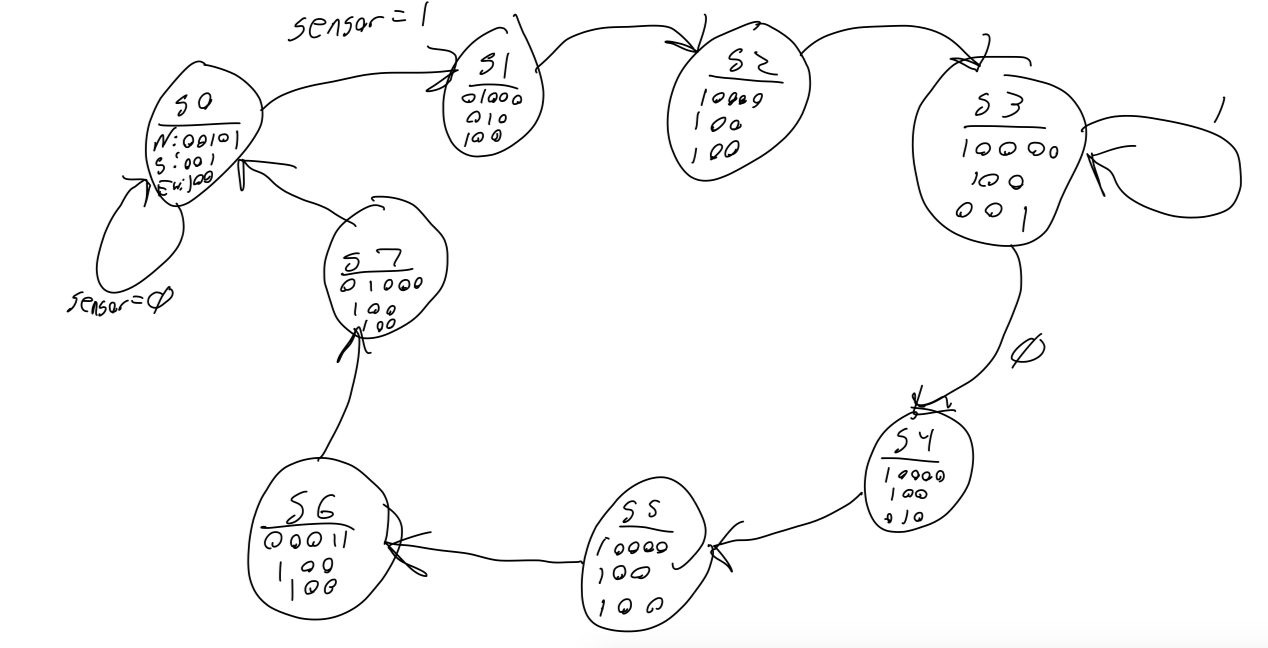
\includegraphics[width=0.5\textwidth]{./images/trafficLightWithTurn.png}
	\caption{\label{fig:part1_state_diagram}State diagram for the traffic controller with a North turn lane.}
\end{center}
\end{figure}

\subsubsection{Results}
The design worked efficiently and as expected. One full cycle is shown in Figures ~\ref{fig:part1_img1} through ~\ref{fig:part1_img9}.

\begin{figure}[H]
\begin{center}
	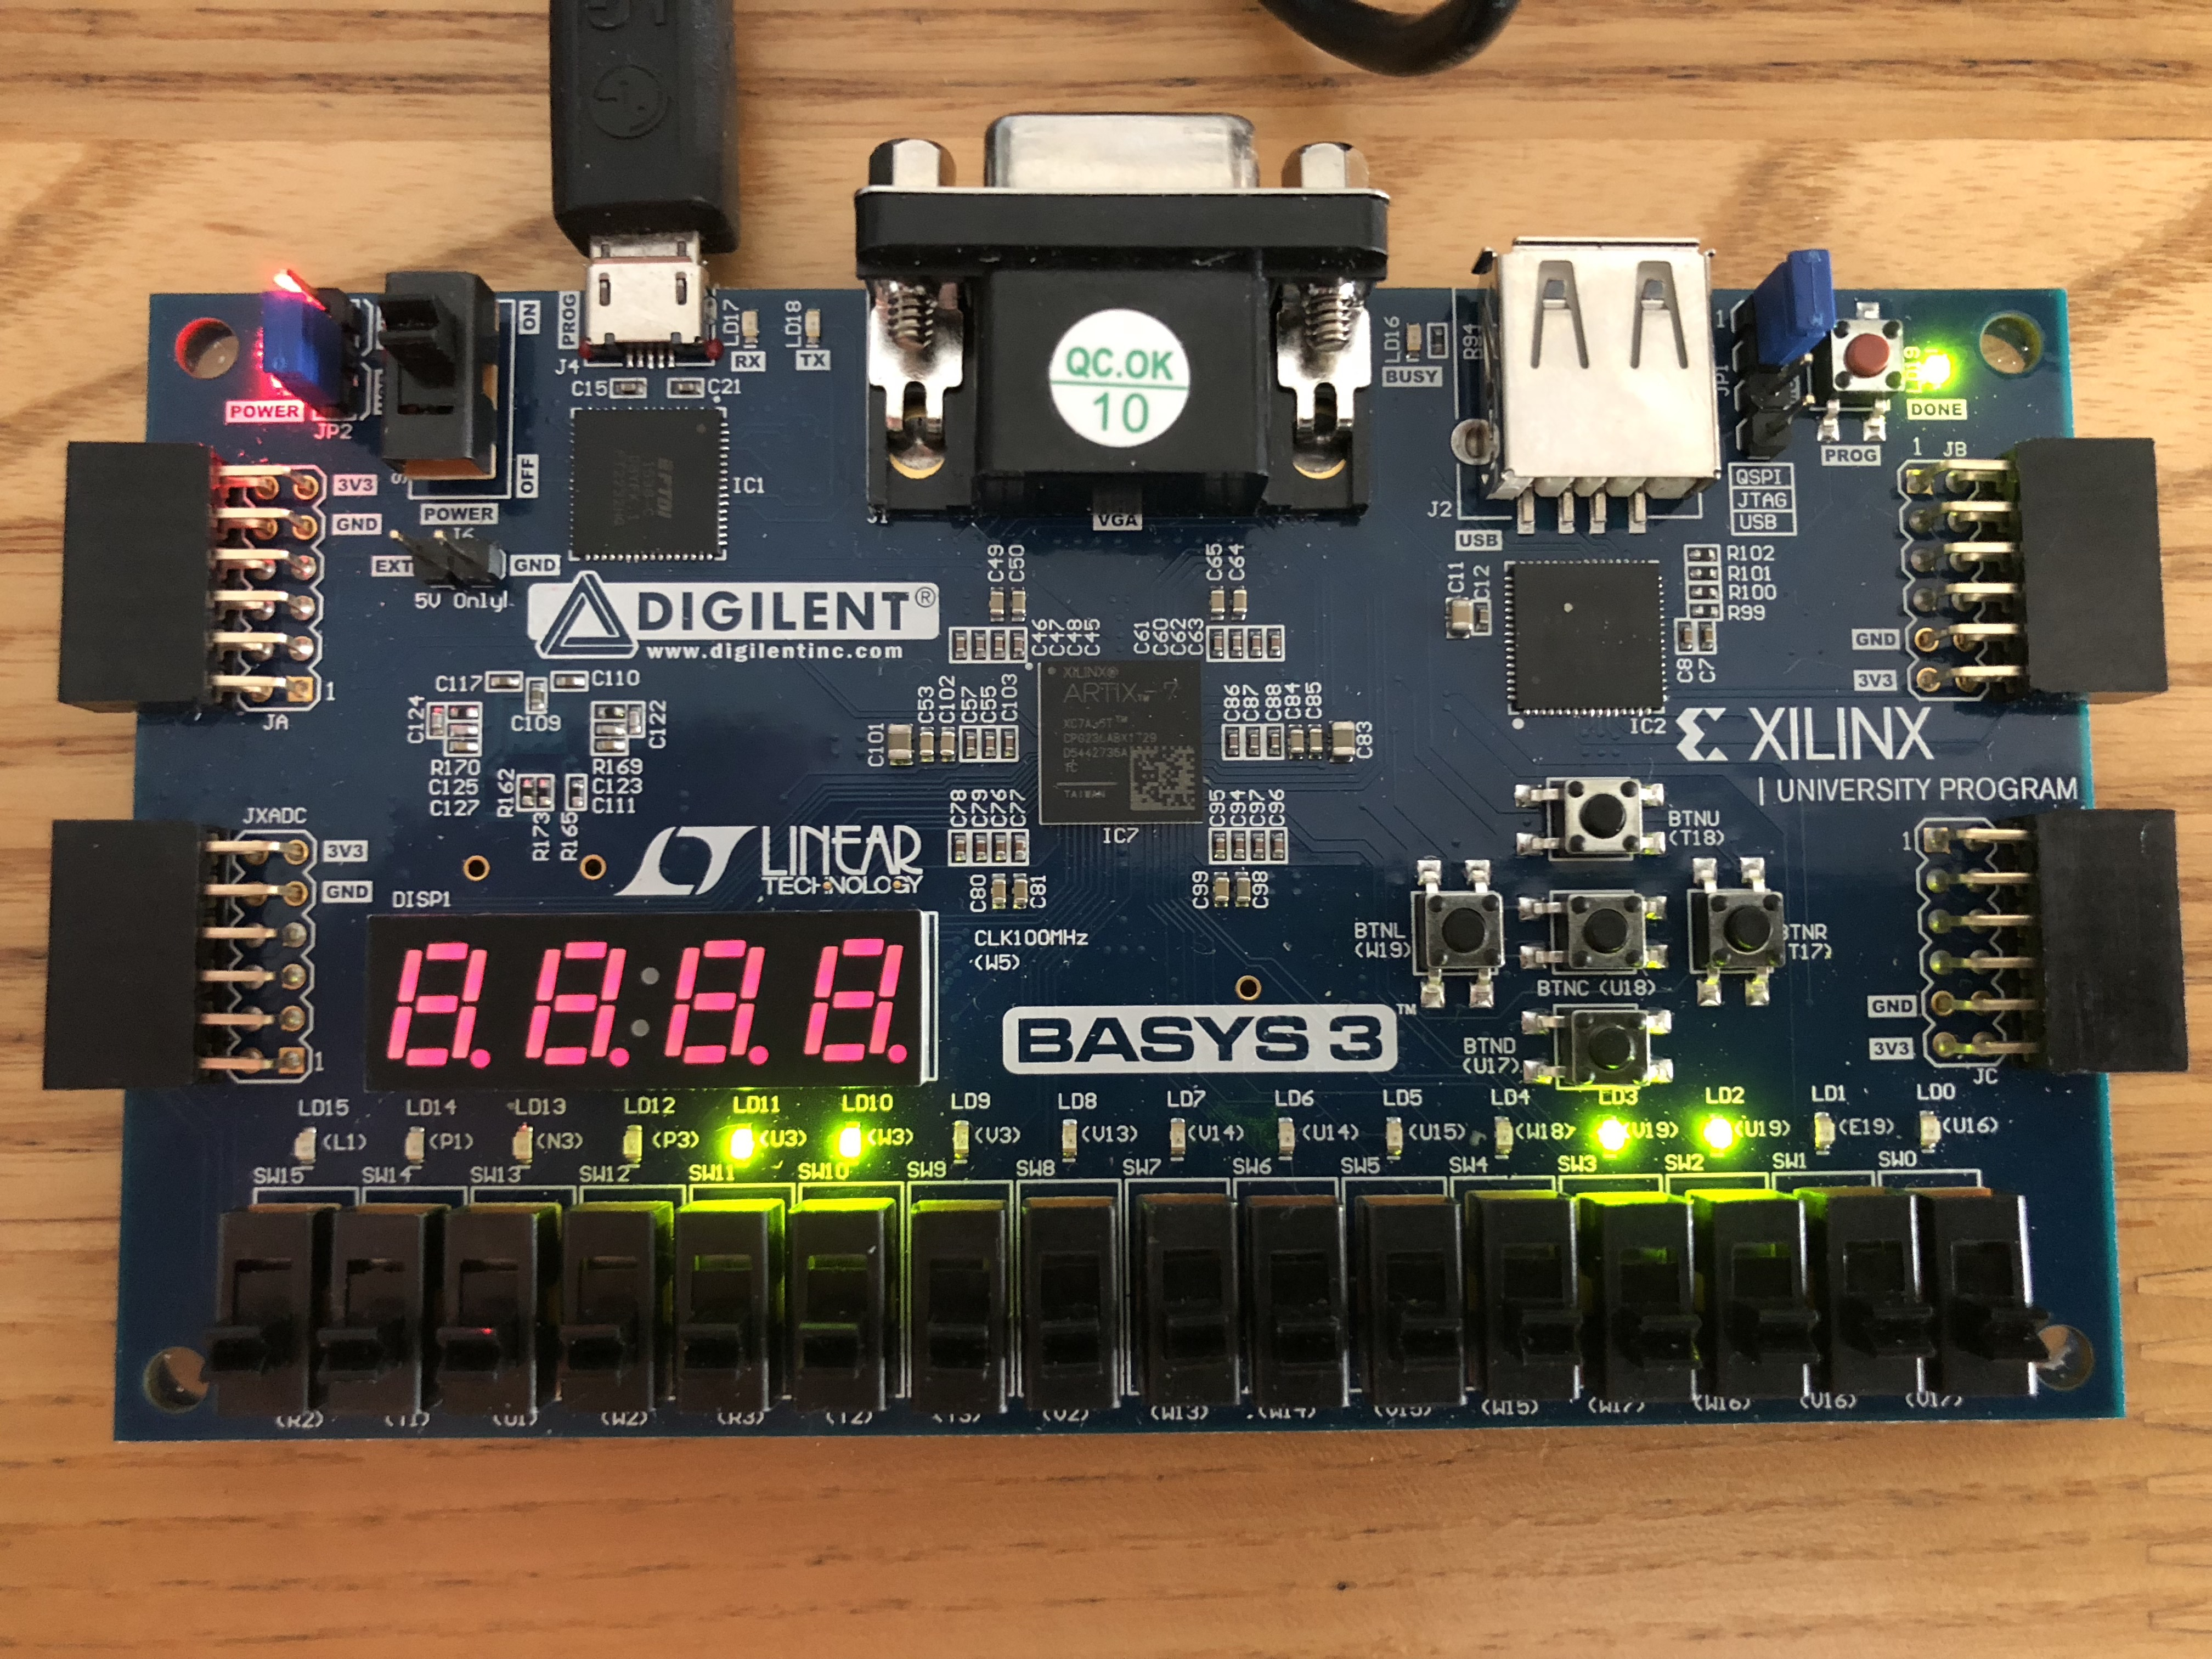
\includegraphics[width=0.5\textwidth]{./images/Part1/l9p1img1.jpg}
	\caption{\label{fig:part1_img1}Standard state, North and South are green, East/West is red.}
\end{center}
\end{figure}

\begin{figure}[H]
\begin{center}
	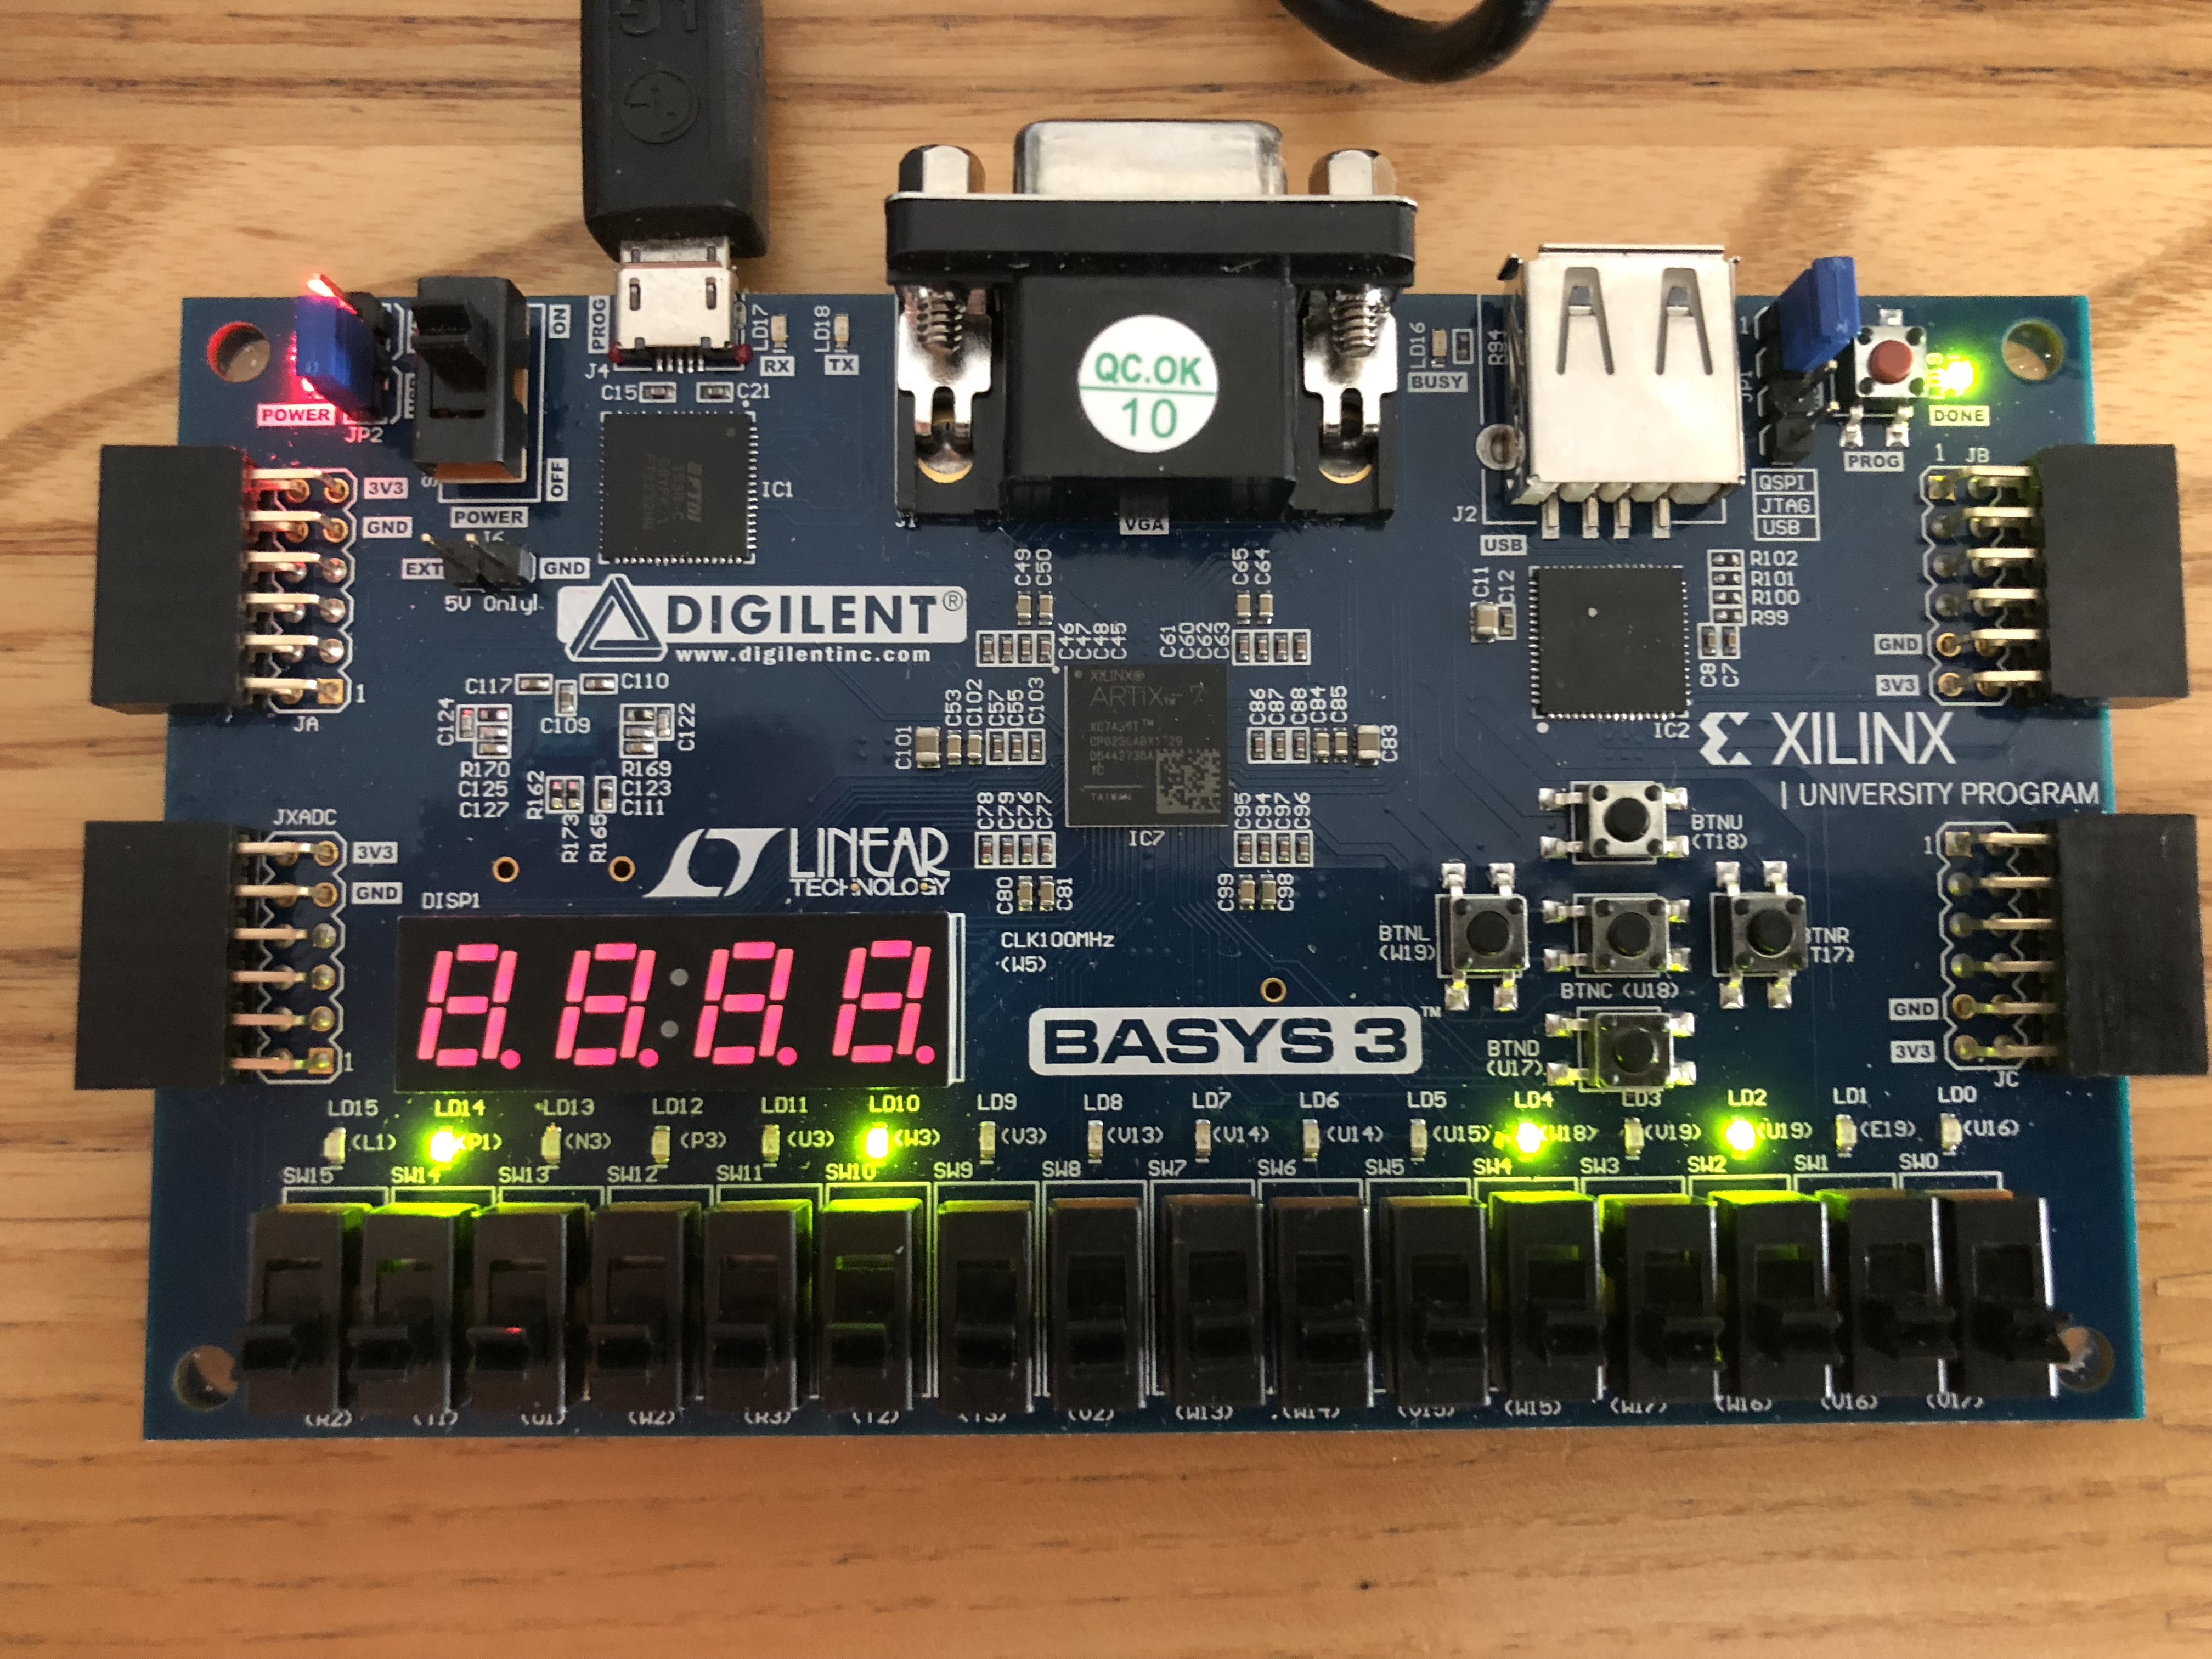
\includegraphics[width=0.5\textwidth]{./images/Part1/l9p1img2.jpg}
	\caption{\label{fig:part1_img2}North and South both turn yellow. East/West still red.}
\end{center}
\end{figure}

\begin{figure}[H]
\begin{center}
	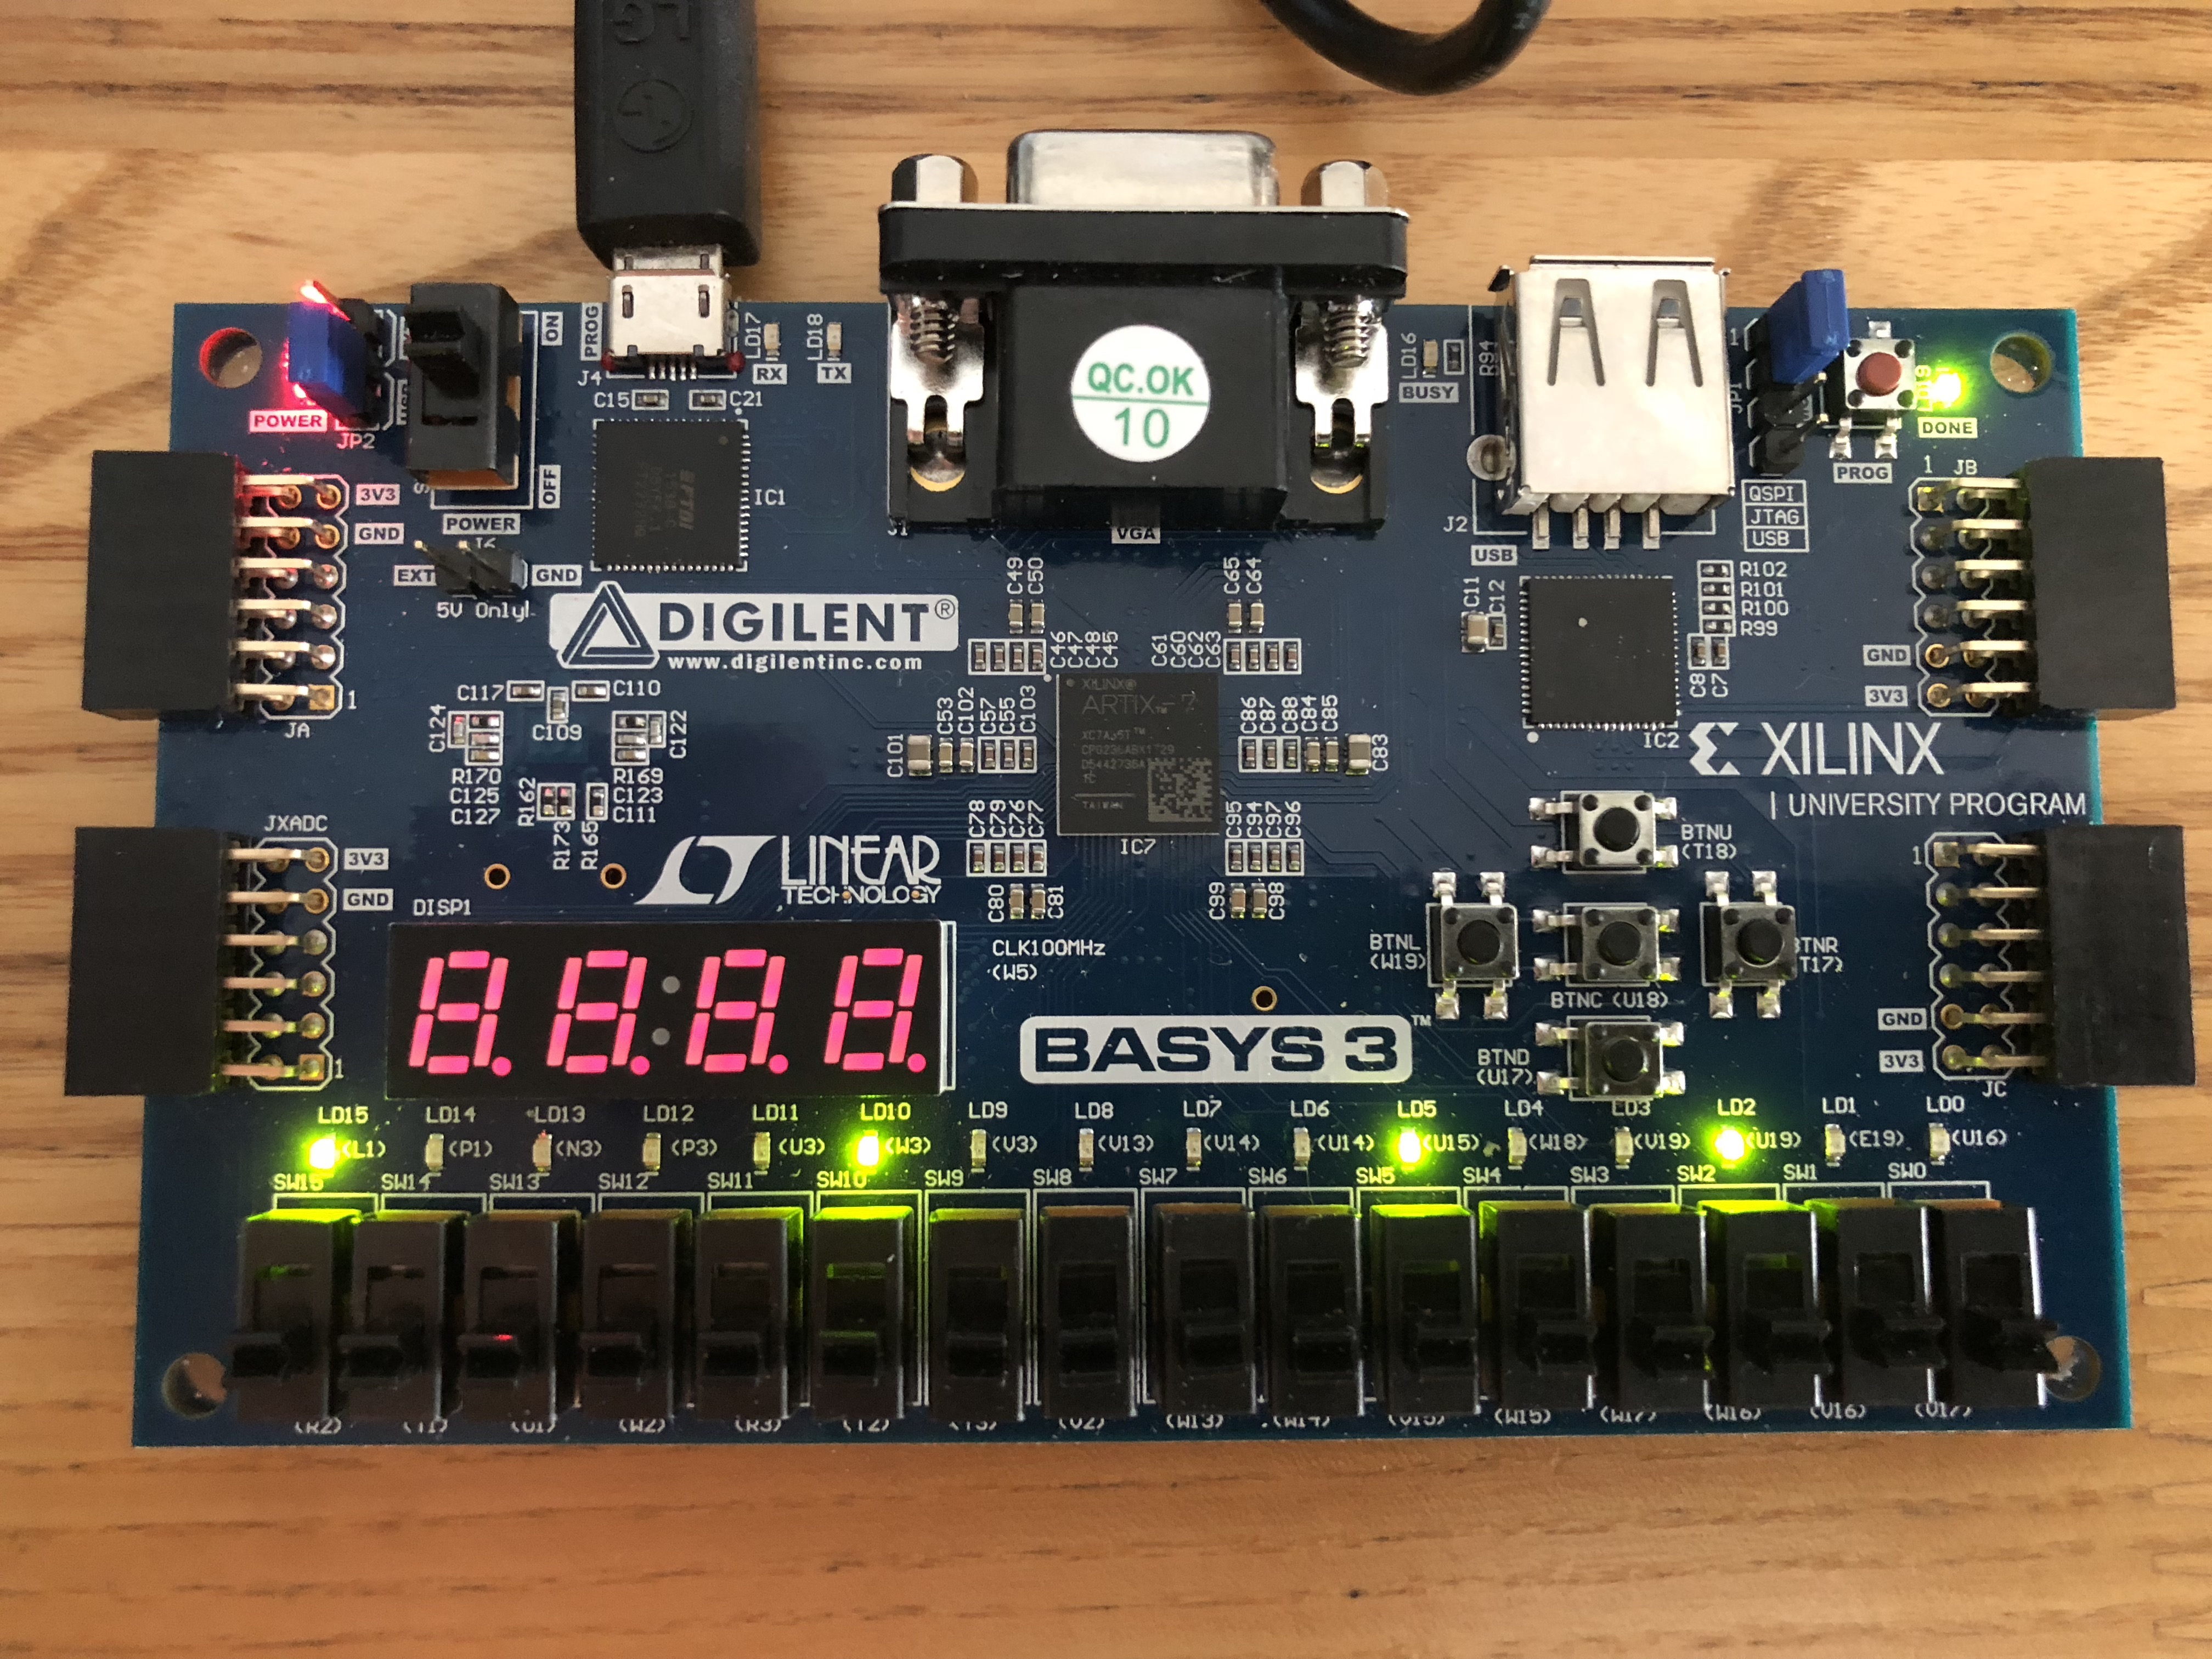
\includegraphics[width=0.5\textwidth]{./images/Part1/l9p1img3.jpg}
	\caption{\label{fig:part1_img3}All lights are red for one cycle before directions change.}
\end{center}
\end{figure}

\begin{figure}[H]
\begin{center}
	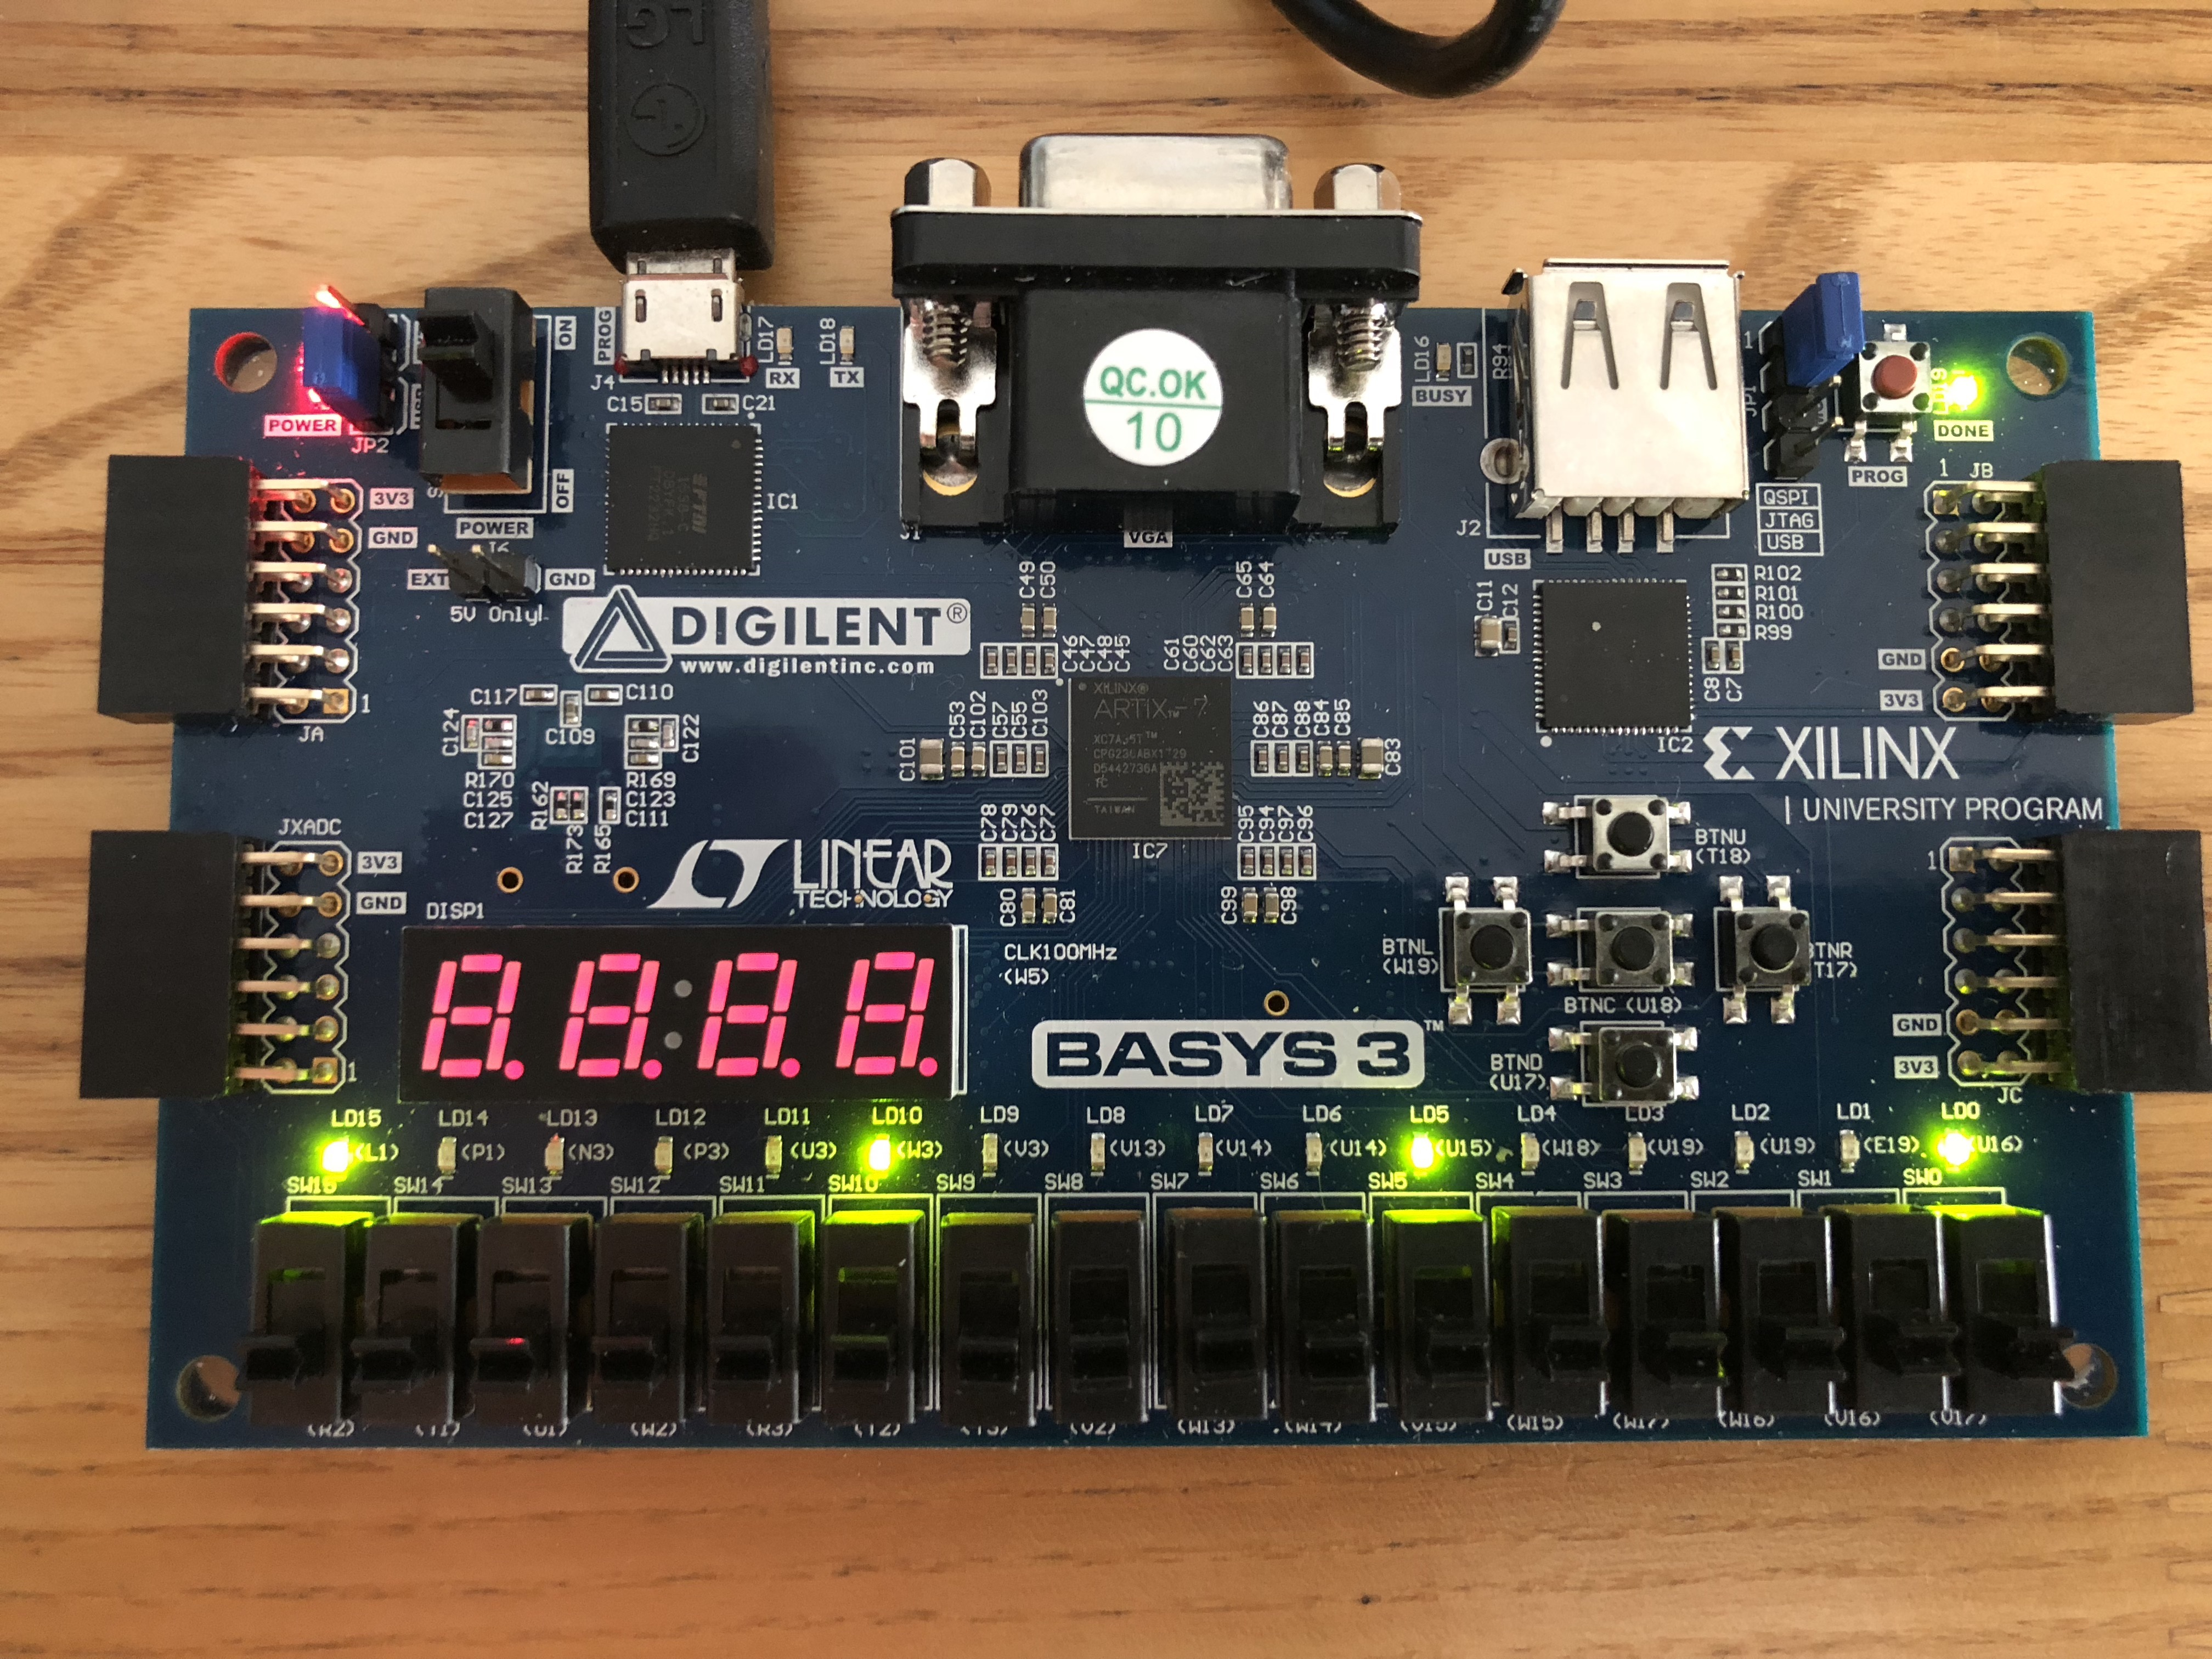
\includegraphics[width=0.5\textwidth]{./images/Part1/l9p1img4.jpg}
	\caption{\label{fig:part1_img4}East/West is green, North and South are both red.}
\end{center}
\end{figure}

\begin{figure}[H]
\begin{center}
	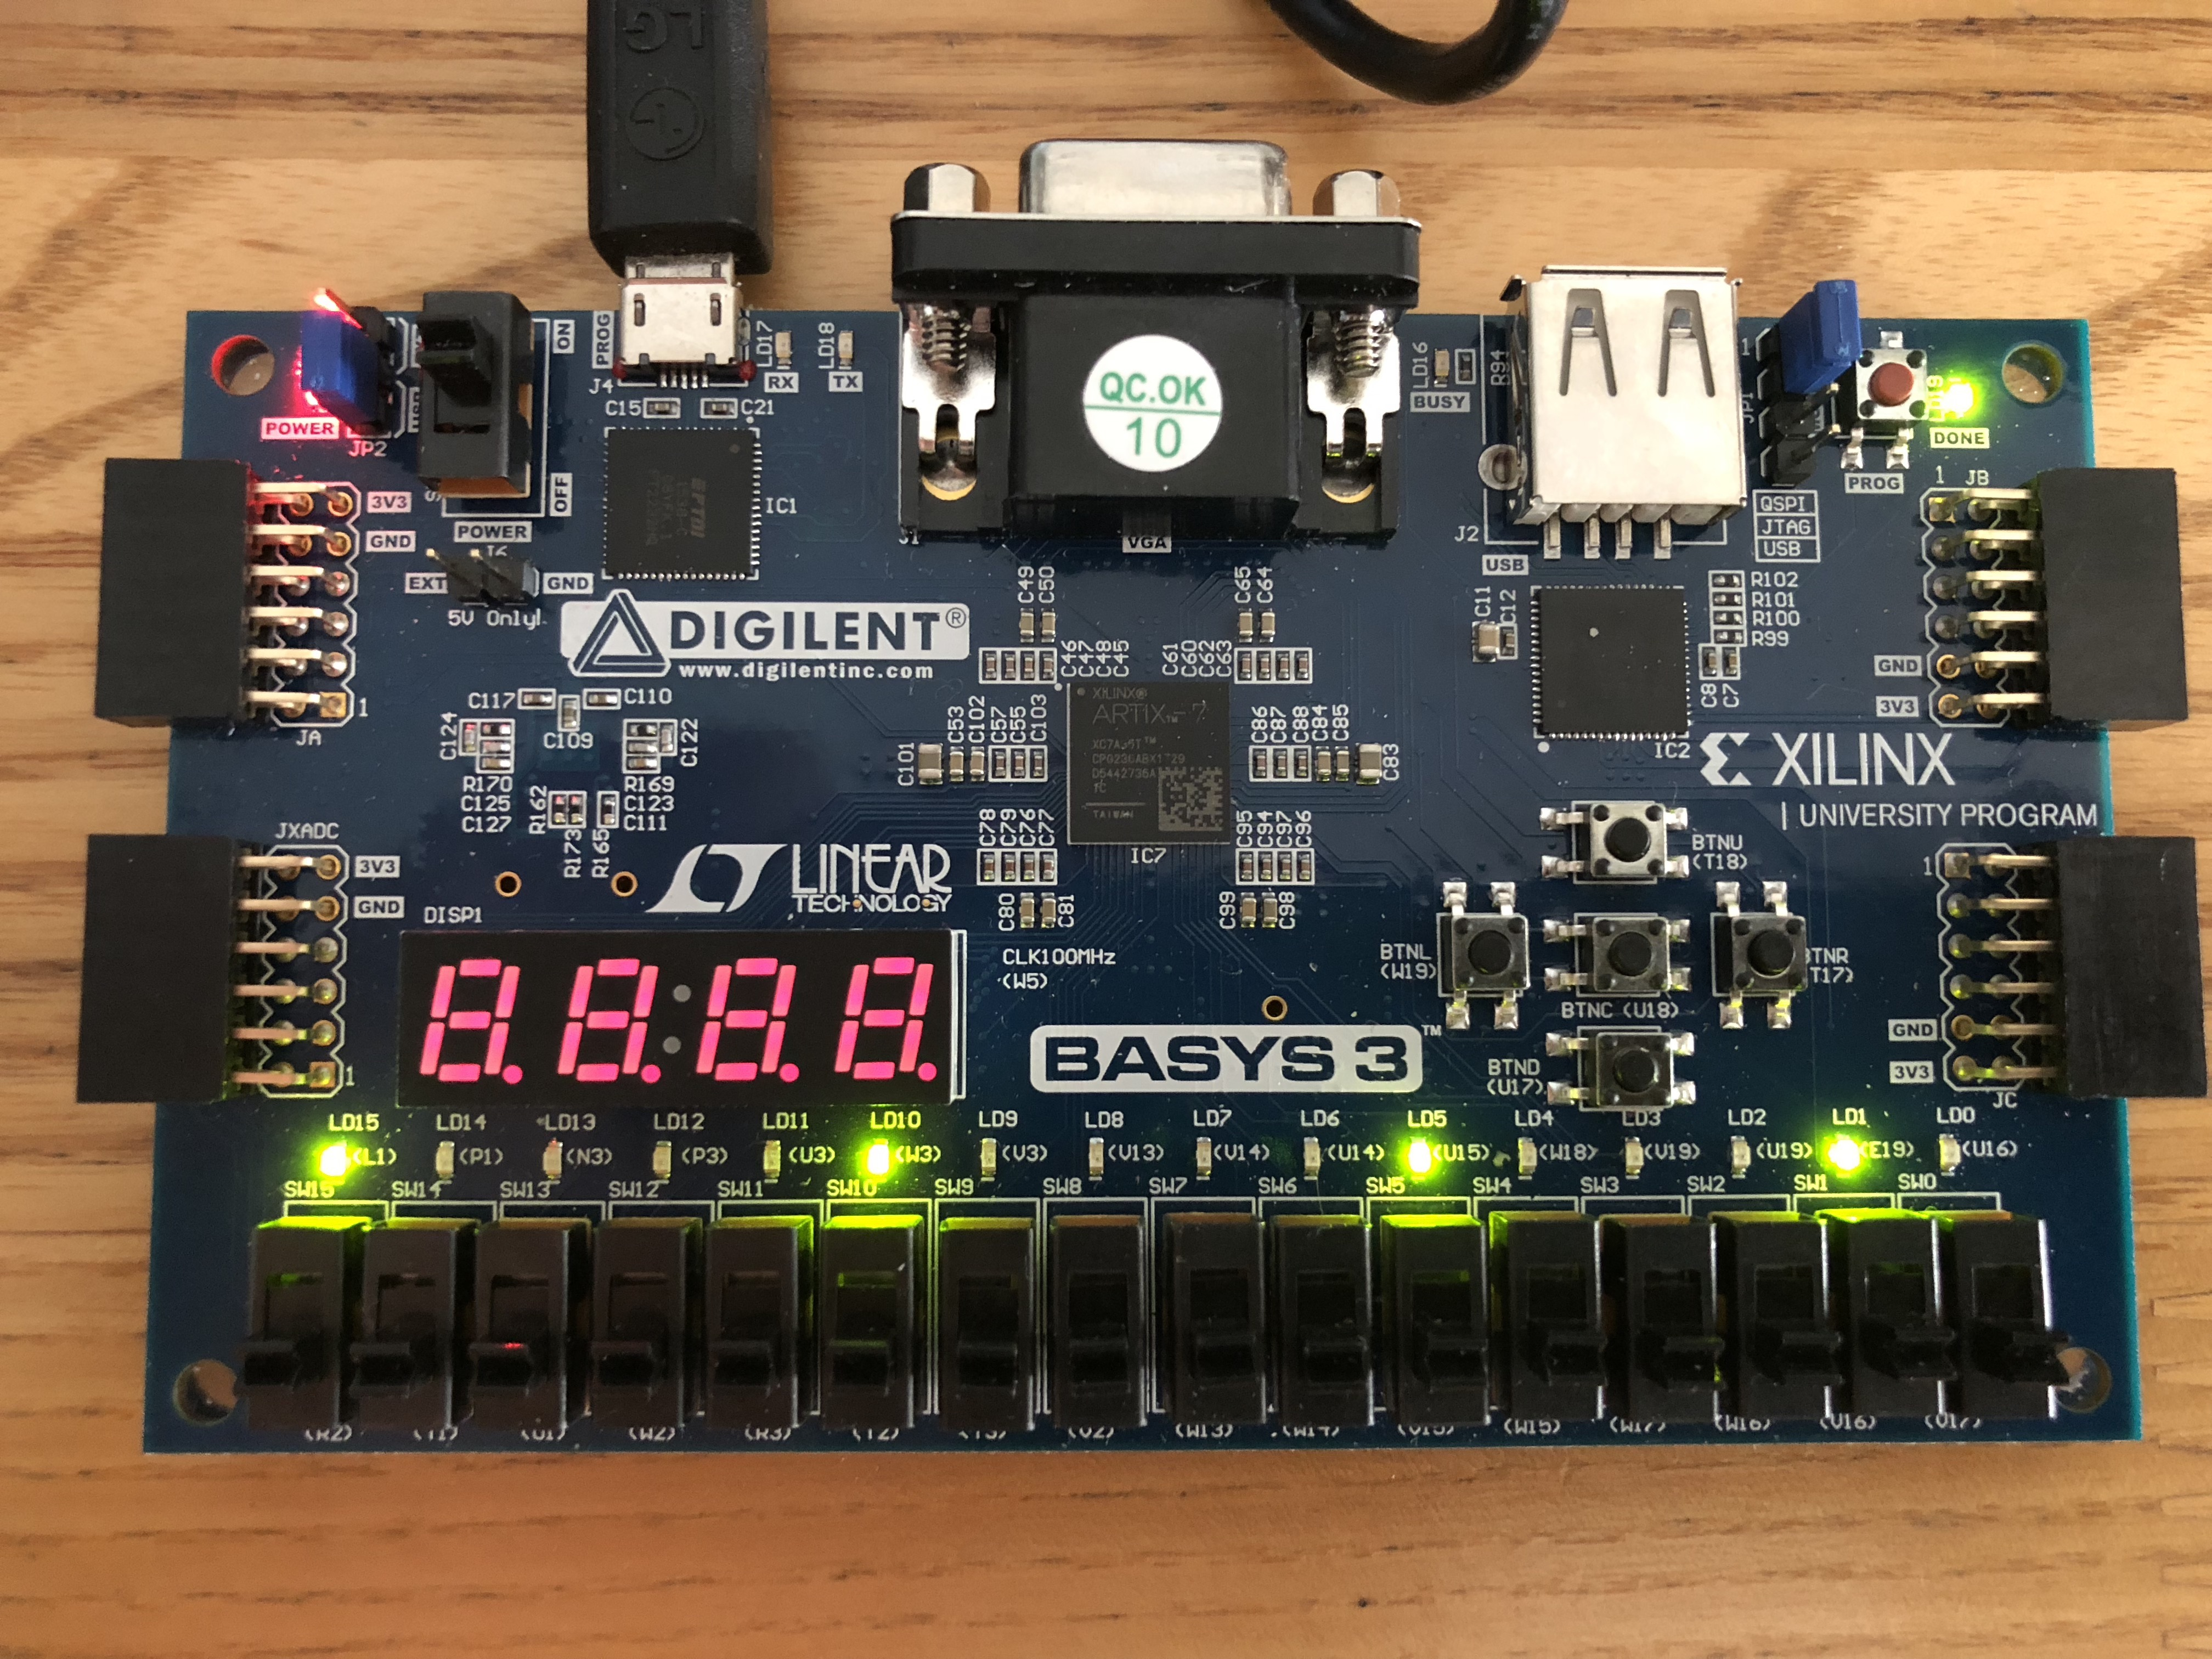
\includegraphics[width=0.5\textwidth]{./images/Part1/l9p1img5.jpg}
	\caption{\label{fig:part1_img5}East/West turns yellow, North and South still red.}
\end{center}
\end{figure}

\begin{figure}[H]
\begin{center}
	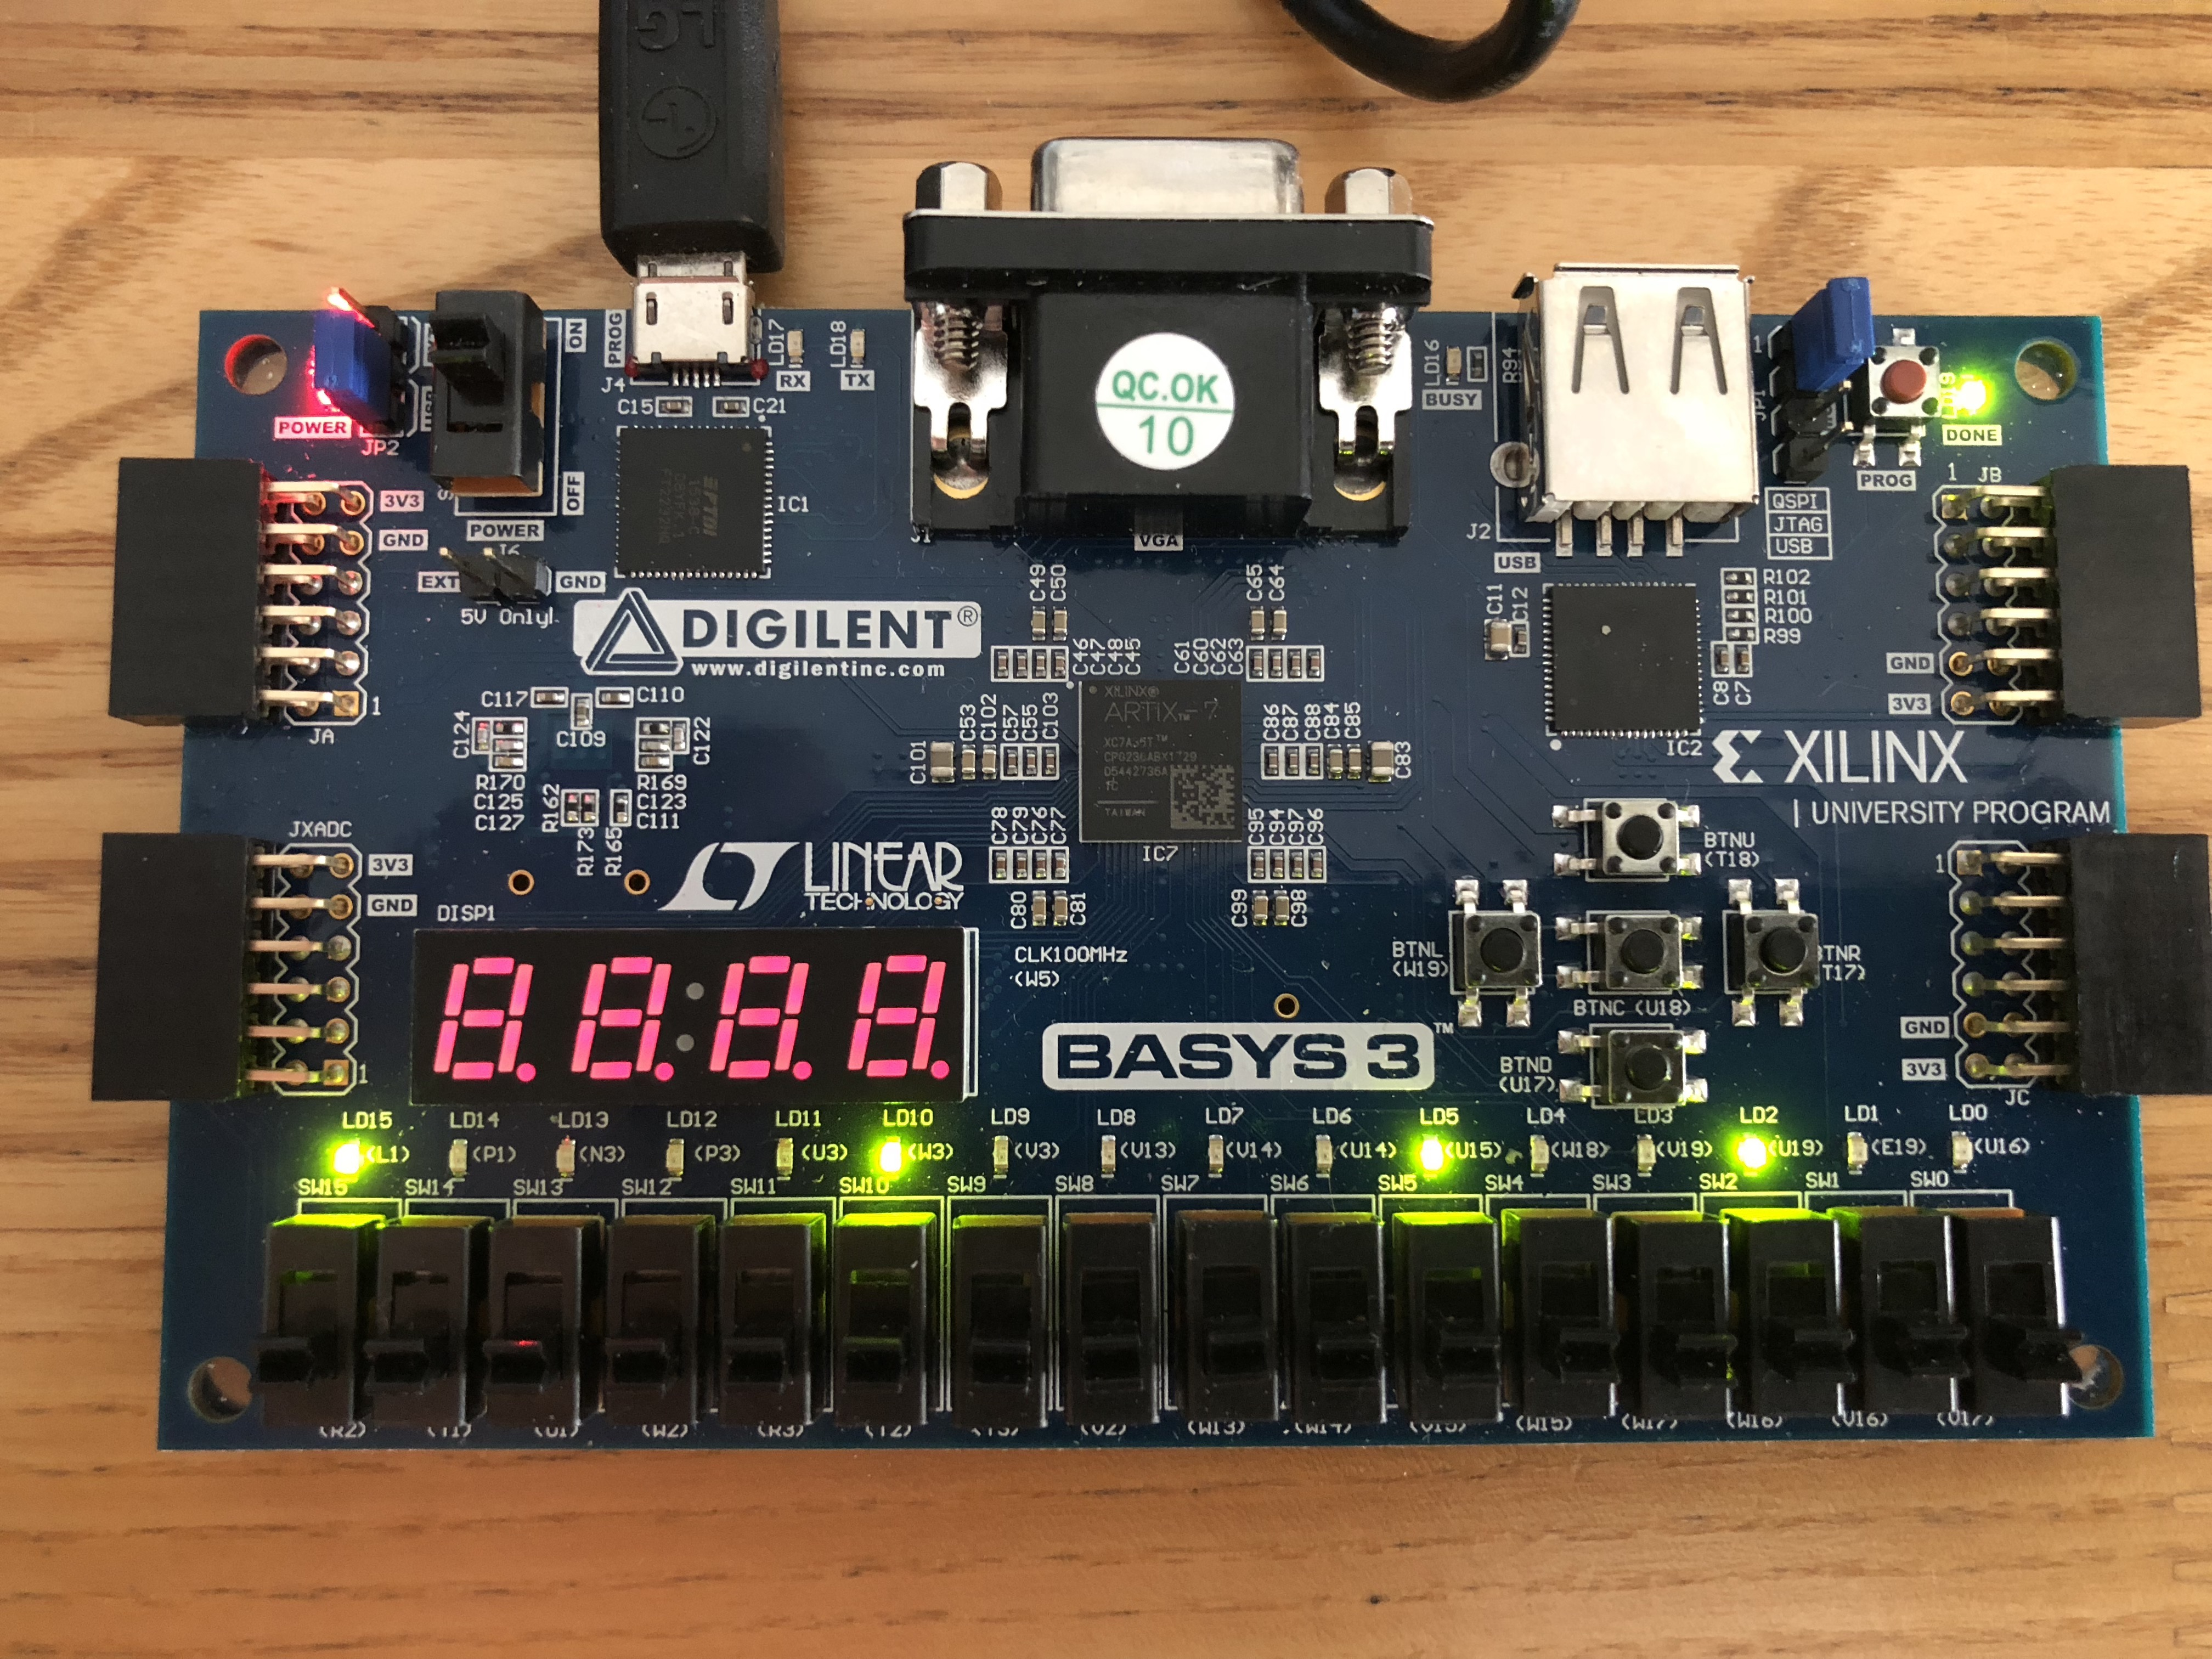
\includegraphics[width=0.5\textwidth]{./images/Part1/l9p1img6.jpg}
	\caption{\label{fig:part1_img6}All lights are red for one cycle before directions change.}
\end{center}
\end{figure}

\begin{figure}[H]
\begin{center}
	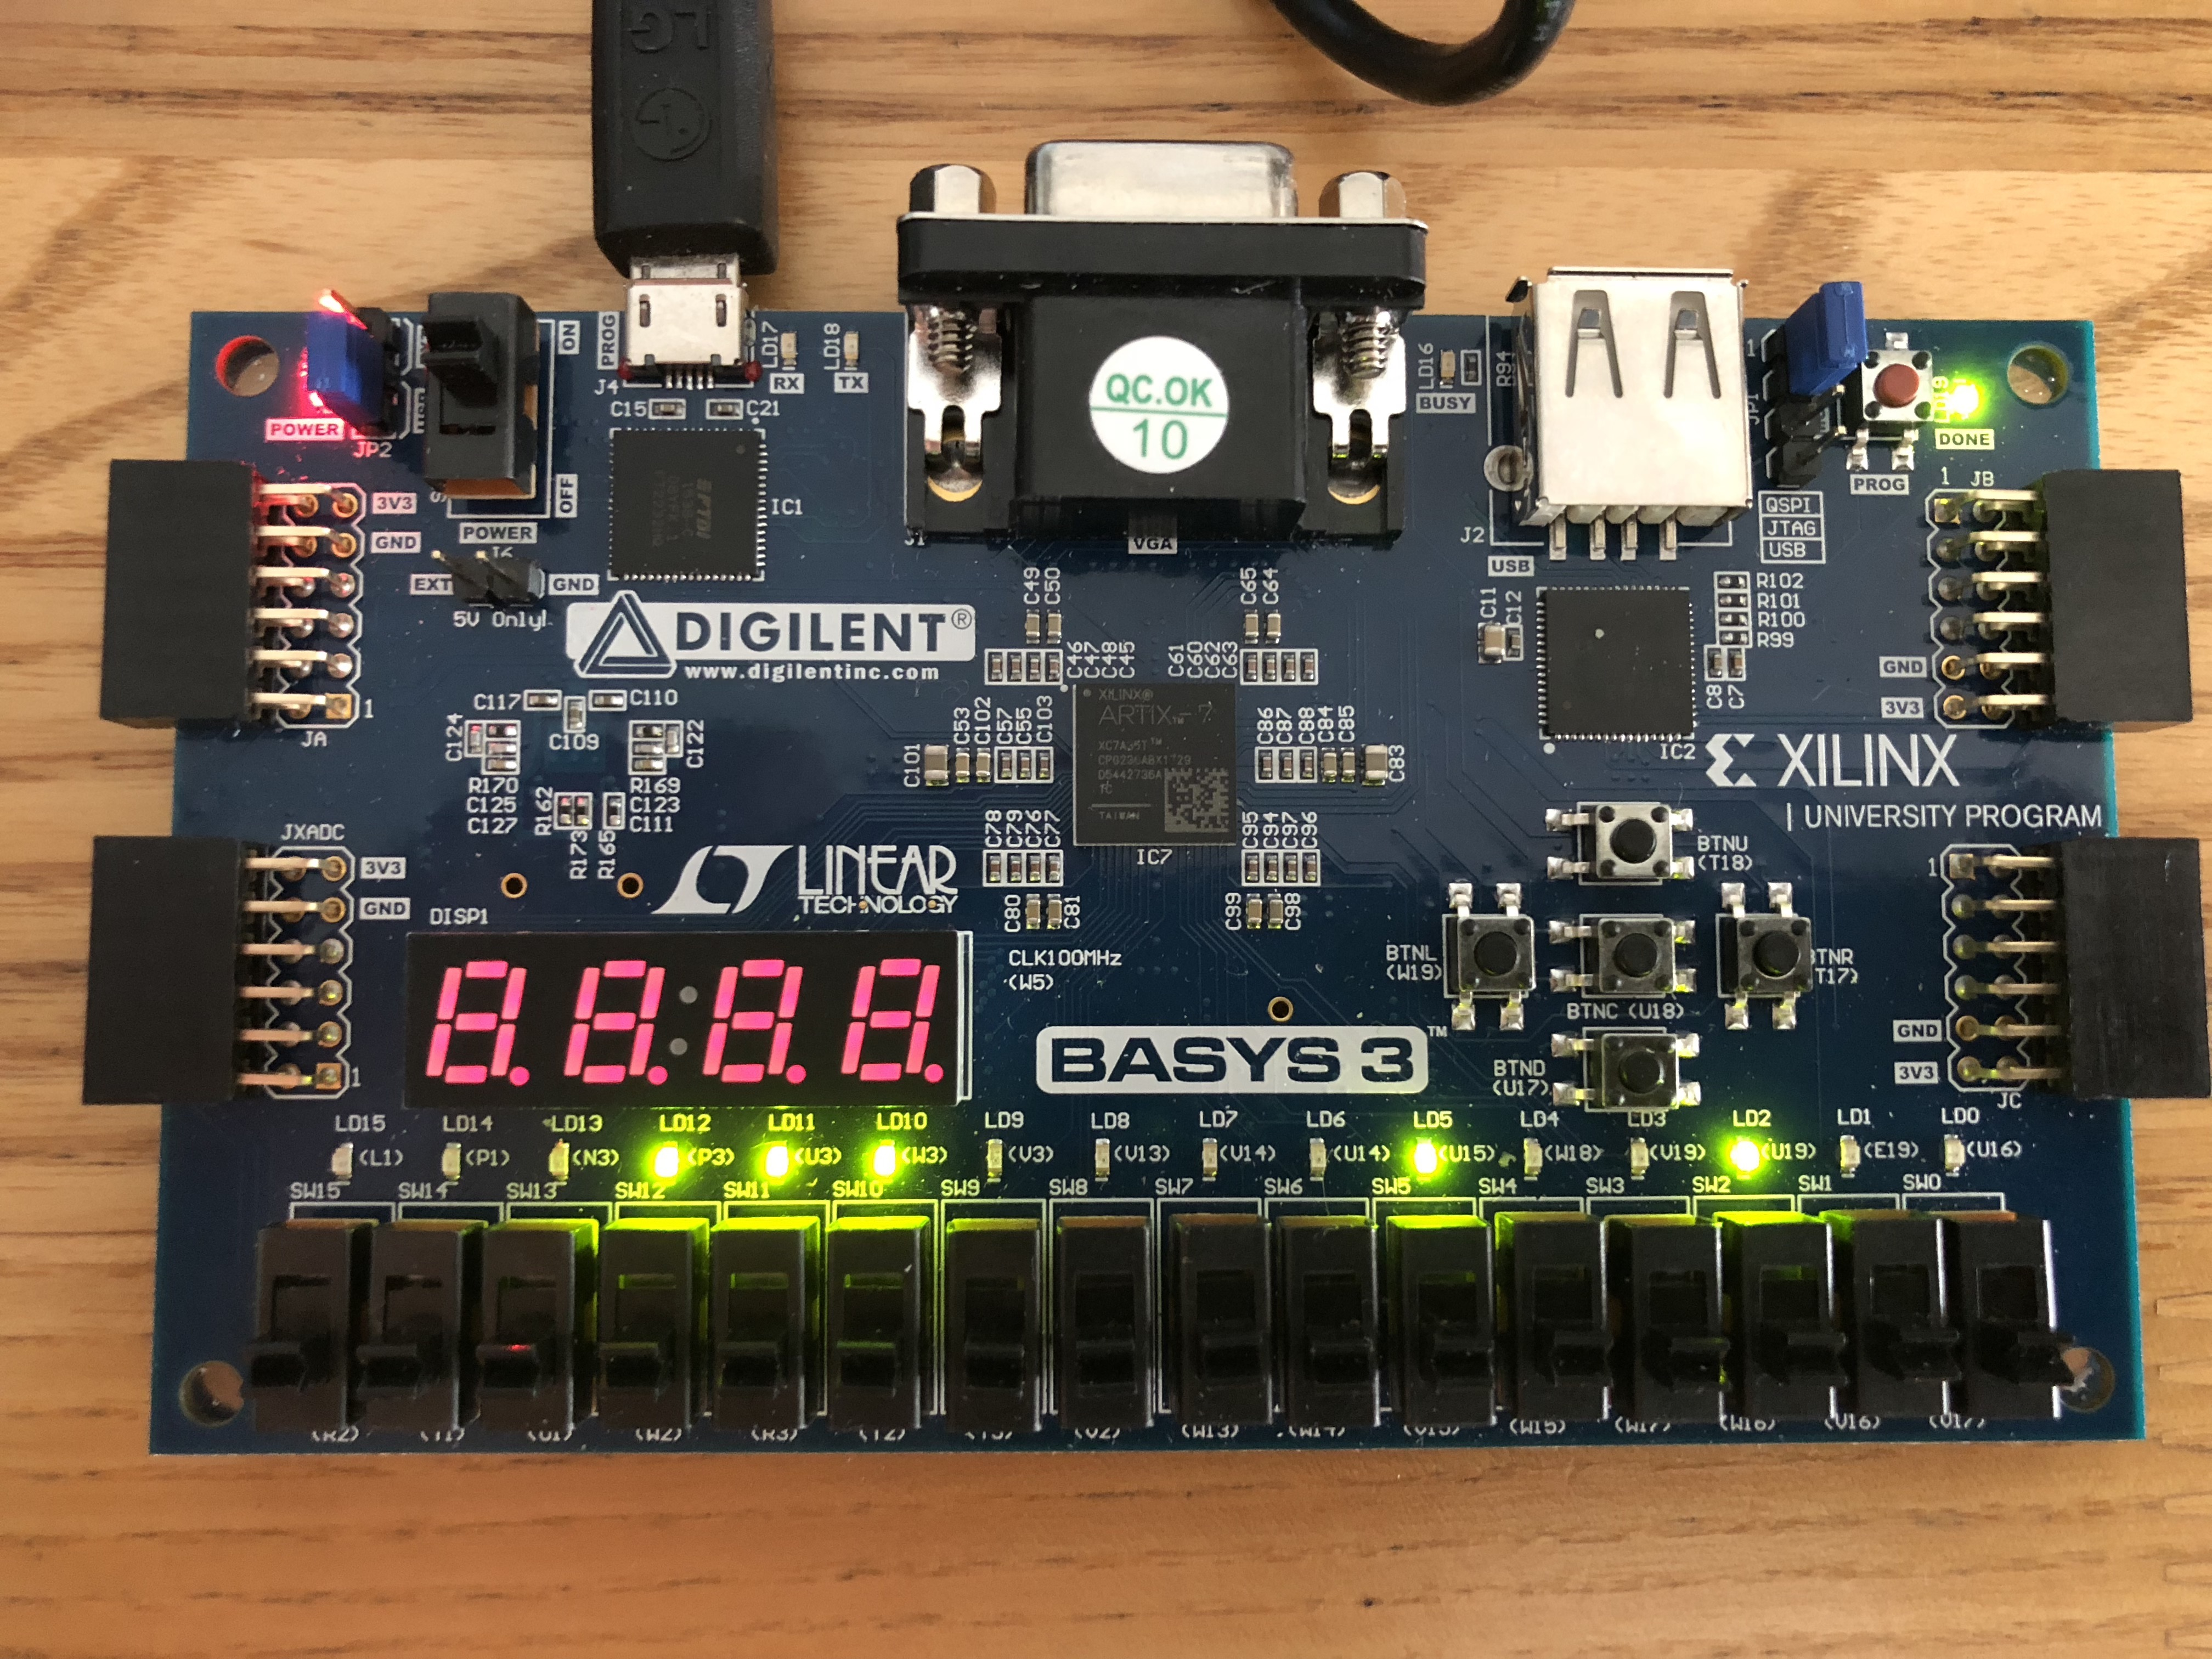
\includegraphics[width=0.5\textwidth]{./images/Part1/l9p1img7.jpg}
	\caption{\label{fig:part1_img7}North and North turn are green, South and East/West are red.}
\end{center}
\end{figure}

\begin{figure}[H]
\begin{center}
	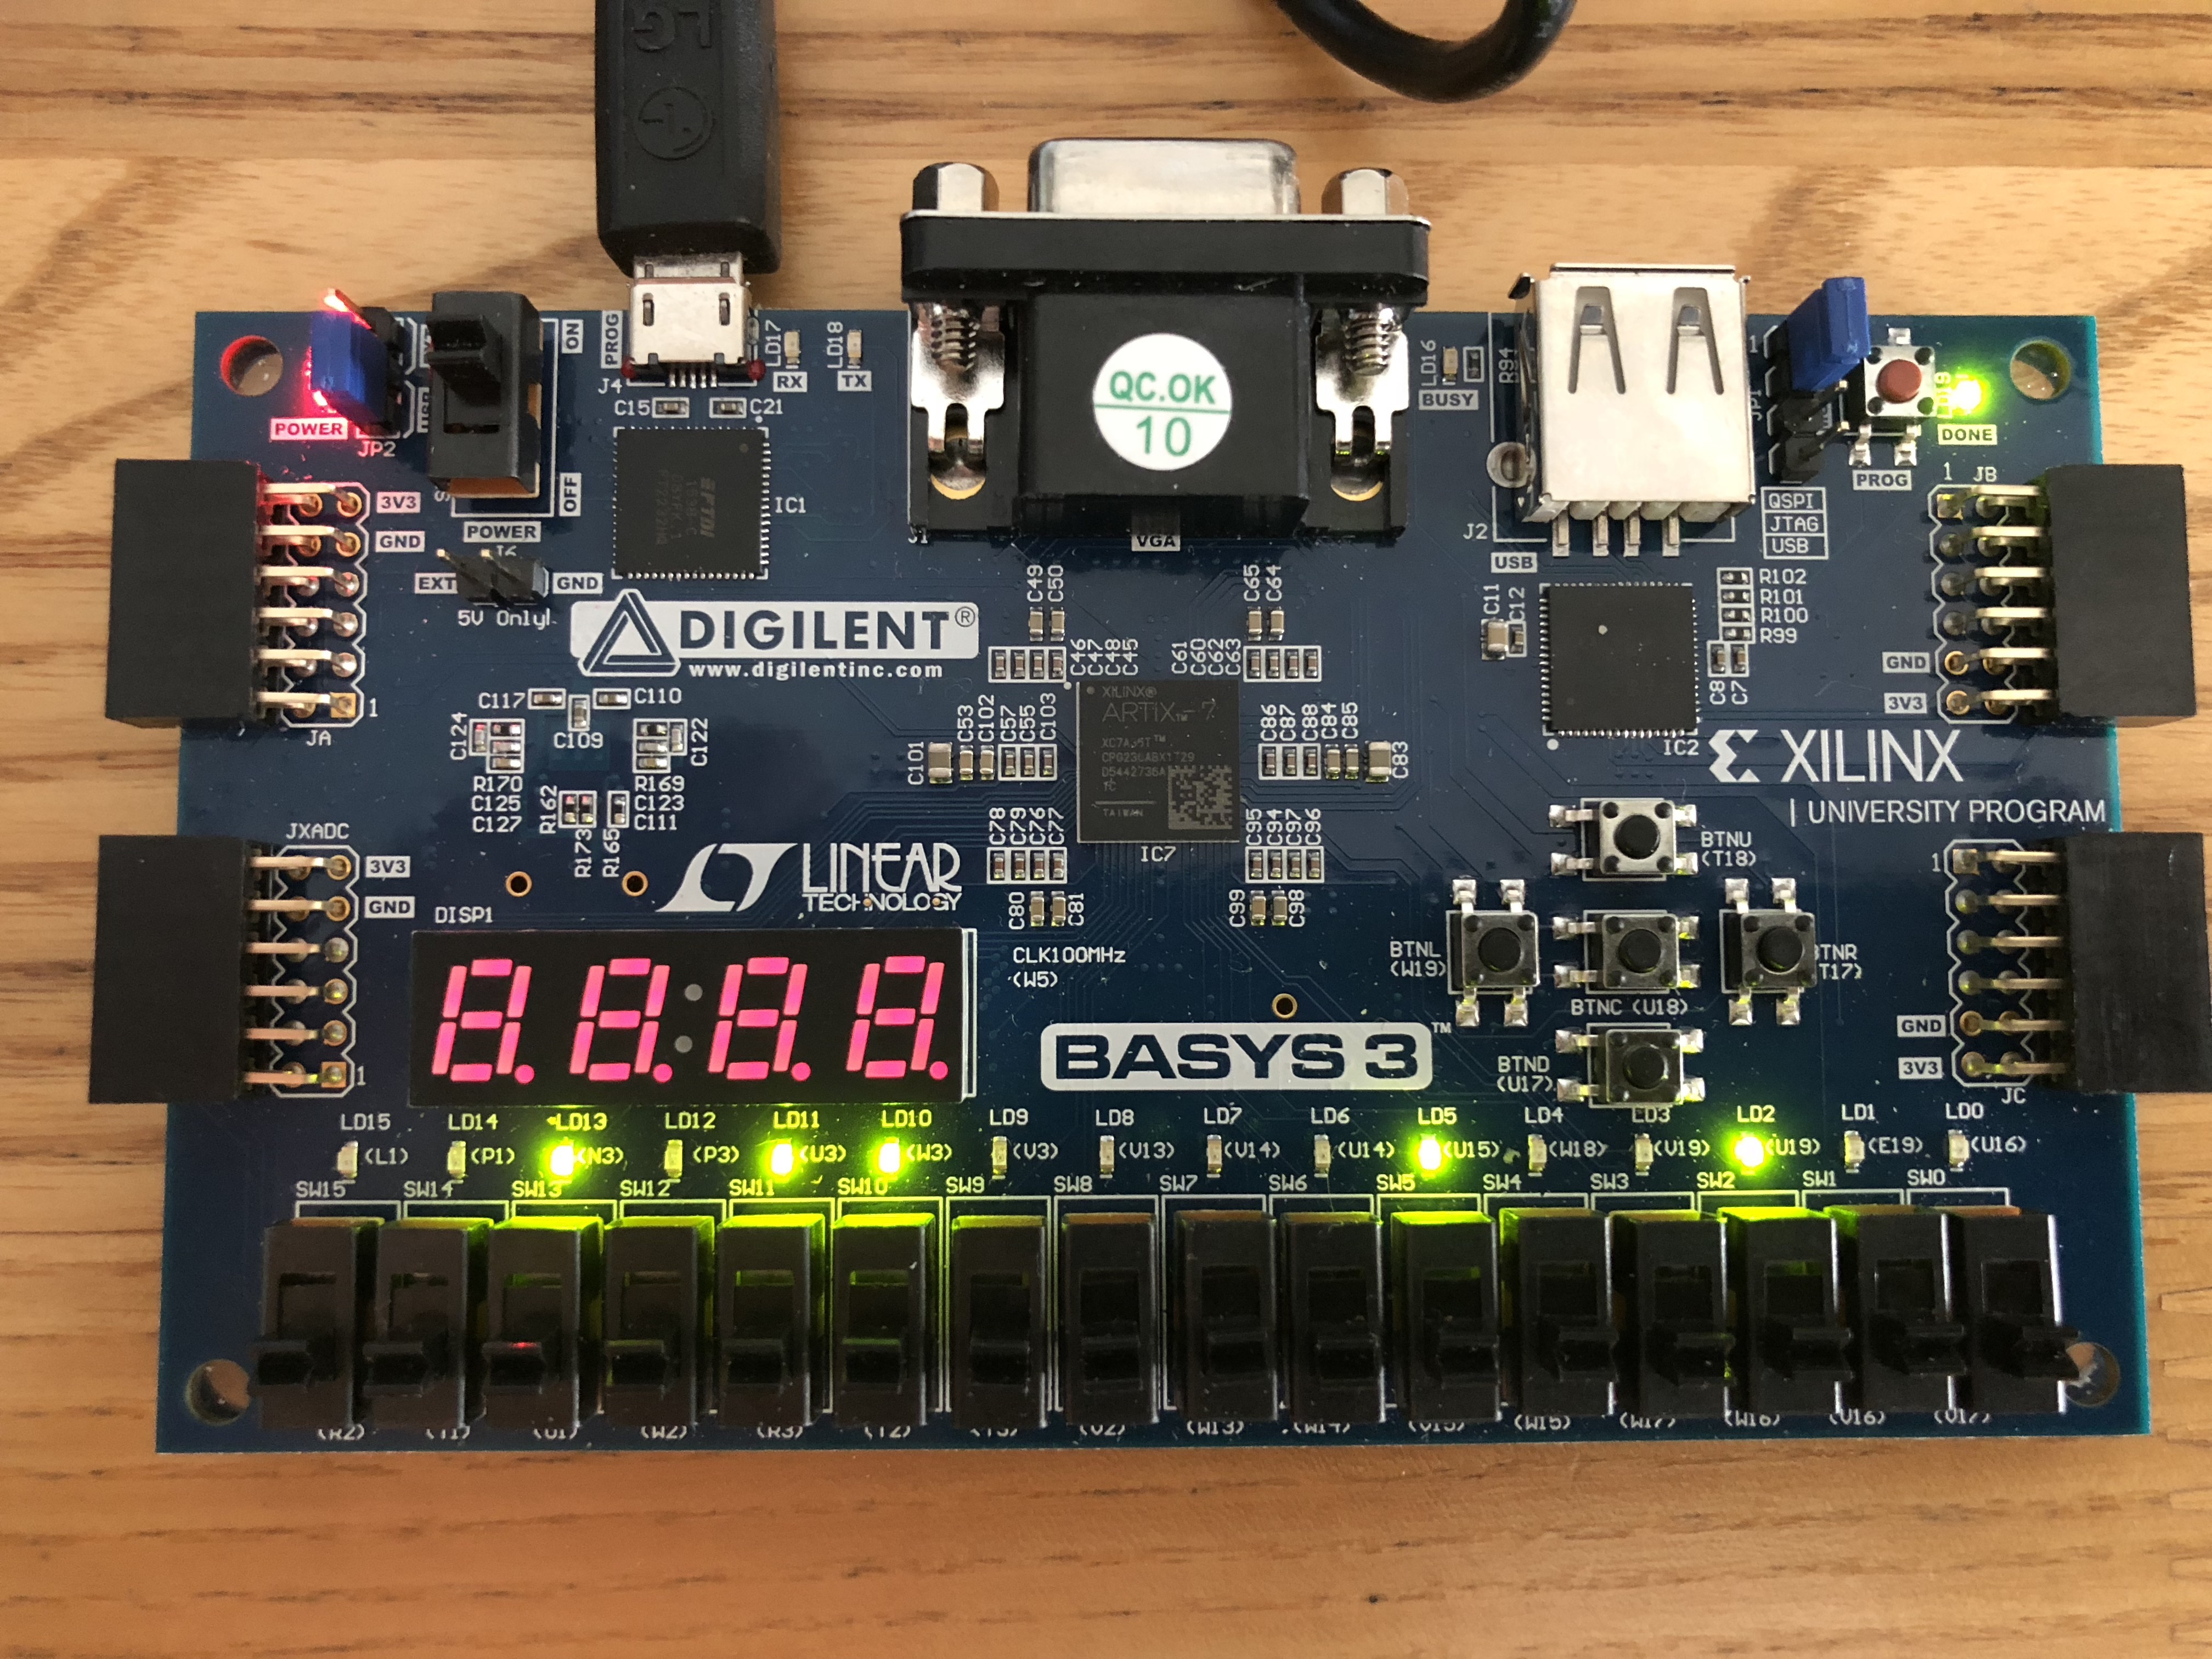
\includegraphics[width=0.5\textwidth]{./images/Part1/l9p1img8.jpg}
	\caption{\label{fig:part1_img8}North is green, North turn is yellow, East/West are red.}
\end{center}
\end{figure}

\begin{figure}[H]
\begin{center}
	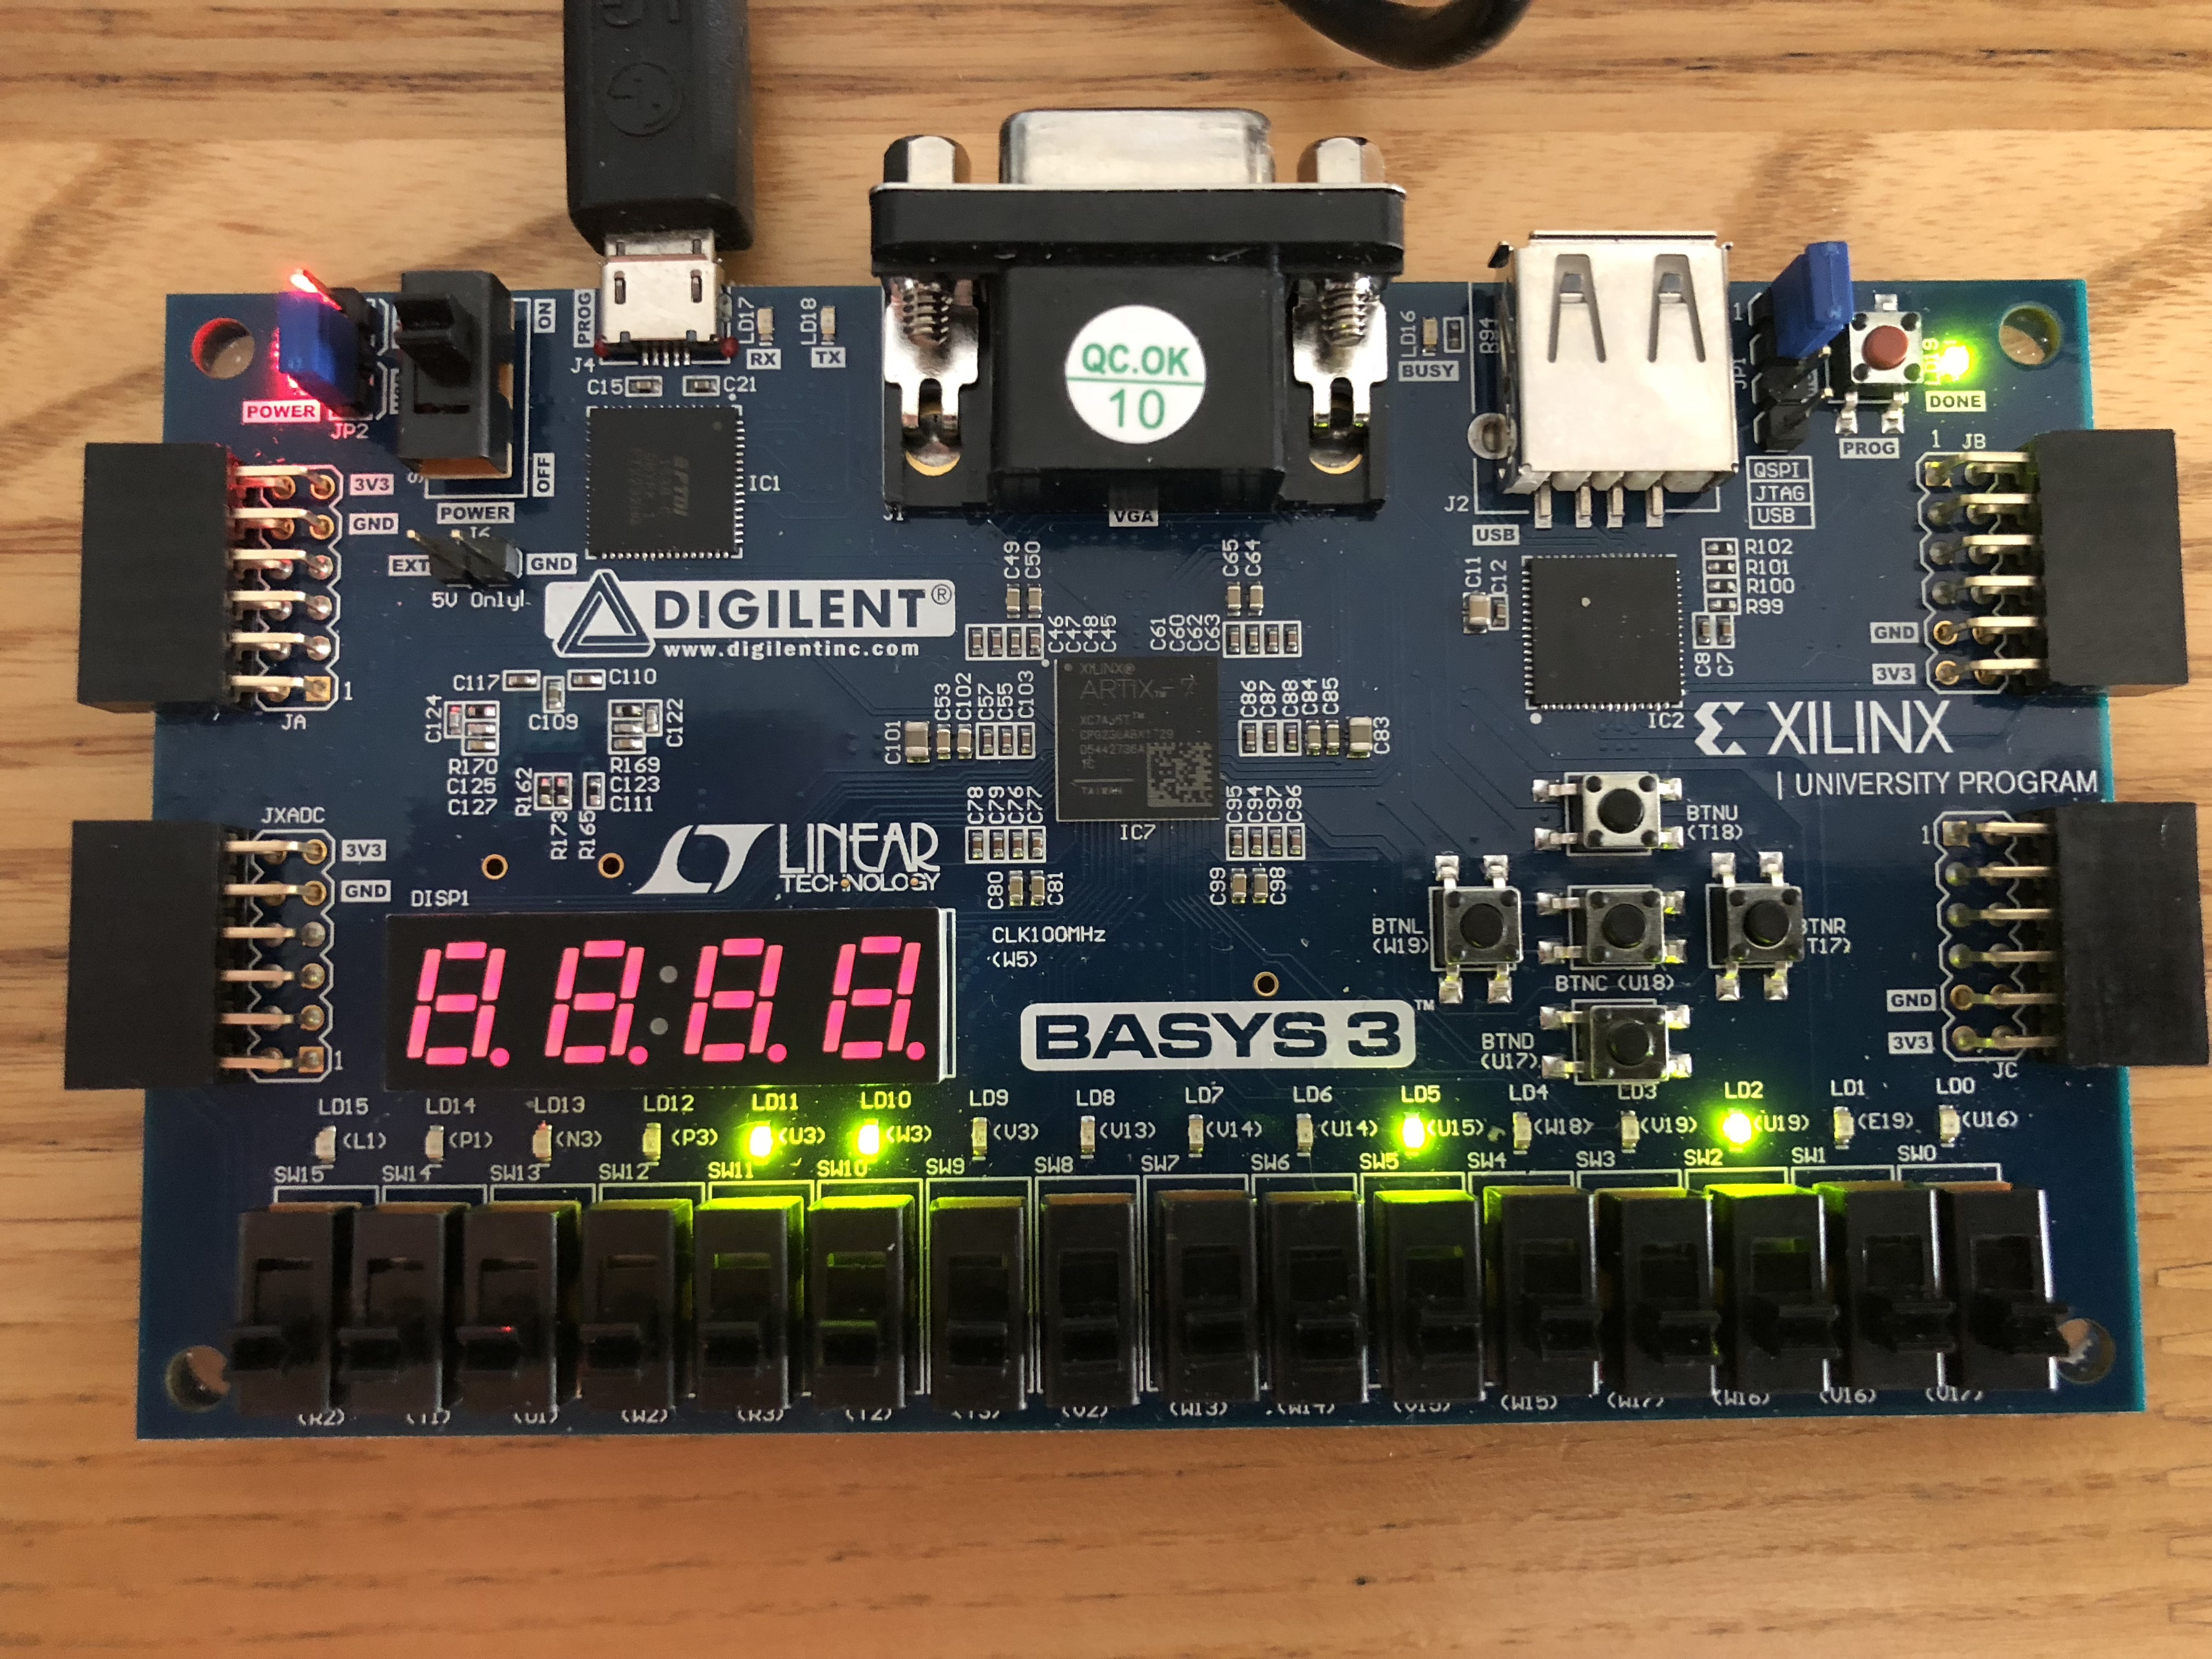
\includegraphics[width=0.5\textwidth]{./images/Part1/l9p1img9.jpg}
	\caption{\label{fig:part1_img9}North is green, wait one cycle before returning to default state.}
\end{center}
\end{figure}


\subsection{Problem 2 }

\subsubsection{Background}
For this problem, we had the same basic state machine with one additional change, we would only go to the North turn green state when a vehicle was detected in the turn lane.

\subsubsection{Design Solution}
Our modified state machine for this problem is shown in Figure ~\ref{fig:part2_state_diagram}. The inputs are summarized in Table ~\ref{tab:part2_input_Ports} and the outputs in Table ~\ref{tab:part2_output_Ports}.

\begin{table}[H]
\begin{center}
\begin{tabular}{| l | l | l |}
	\hline
	Bit & Label & Port \\ \hline
	clk &  Clock & W5 \\ \hline
	reset & Button Center & U18 \\ \hline
	sensor EW 1 Swtch 0 & & V17 \\ \hline
	sensor EW 0 & Switch 1 & V16 \\ \hline
	sensor NT & Button Right& T17 \\ \hline
\end{tabular}
\caption{\label{tab:part2_input_Ports}Input port assignments for  the second traffic system.}
\end{center}
\end{table}

\begin{table}[H]
\begin{center}
\begin{tabular}{| l | l | l |}
	\hline
	Bit & Label & Port \\ \hline
	clk led & LED 12 & P3 \\ \hline
	east west 2 & LED 15 & L1 \\ \hline
	east west 1 & LED 14 & P1 \\ \hline
	east west 0 & LED 13 & N3 \\ \hline
	south 2 & LED 11 & U3 \\ \hline
	south 1 & LED 10 & W3 \\ \hline
	south 0 & LED 9 & V3 \\ \hline
	north 4 & LED 4 & W18 \\ \hline
	north 3 & LED 3 & V19 \\ \hline
	north 2 & LED 2 & U19 \\ \hline
	north 1 & LED 1 & E19 \\ \hline
	north 0 & LED 0 & U16 \\ \hline
\end{tabular}
\caption{\label{tab:part2_output_Ports}Output port assignments for the second traffic system.}
\end{center}
\end{table}

\begin{figure}
\begin{center}
	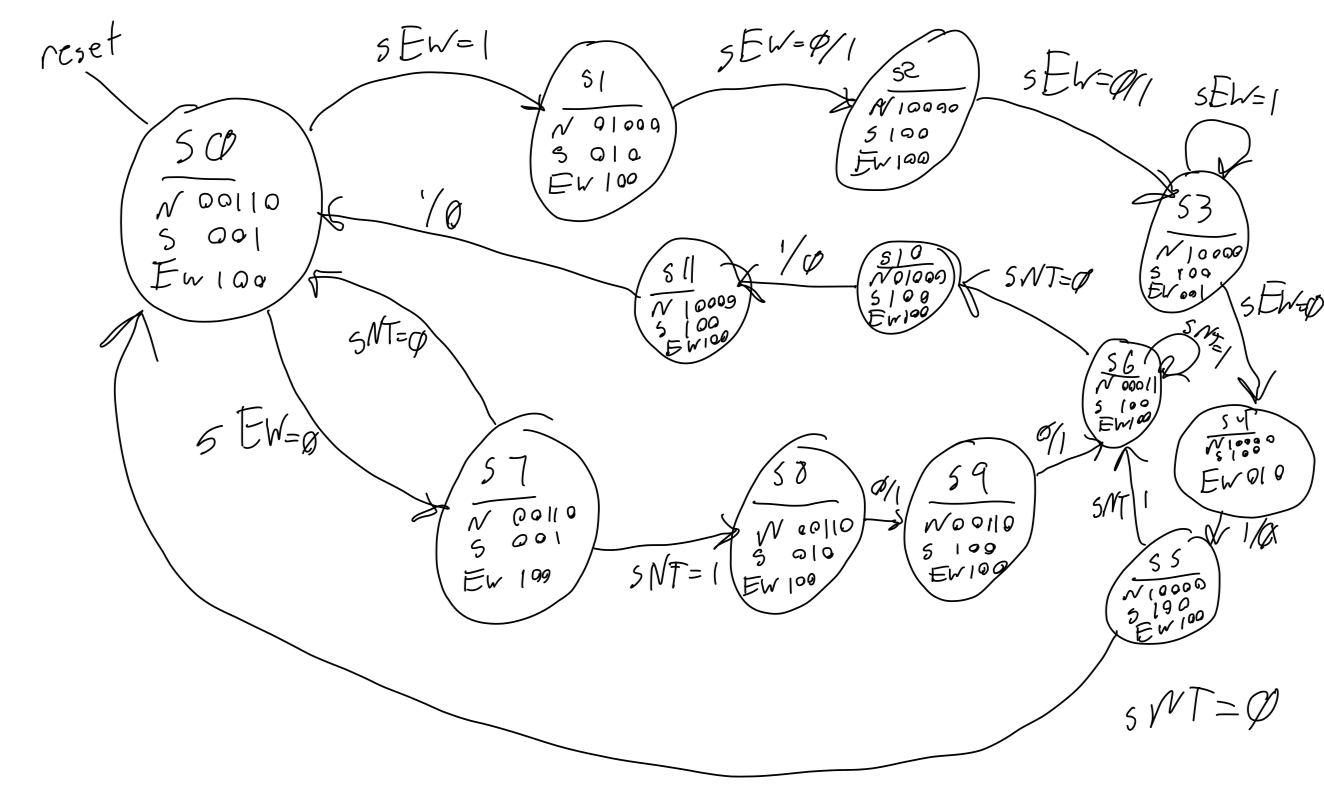
\includegraphics[width=0.5\textwidth]{./images/trafficLightWithSensorTurn.png}
	\caption{\label{fig:part2_state_diagram}State diagram for the traffic controller with a North turn lane managed by a sensor.}
\end{center}
\end{figure}


\subsubsection{Results}
This design worked as expected and fulfilled all requirements. Since the East/West traffic flow is the same as the previous problem, only the new North turn process is shown in Figures ~\ref{fig:part2_img1} through ~\ref{fig:part2_img6}.

\begin{figure}[H]
\begin{center}
	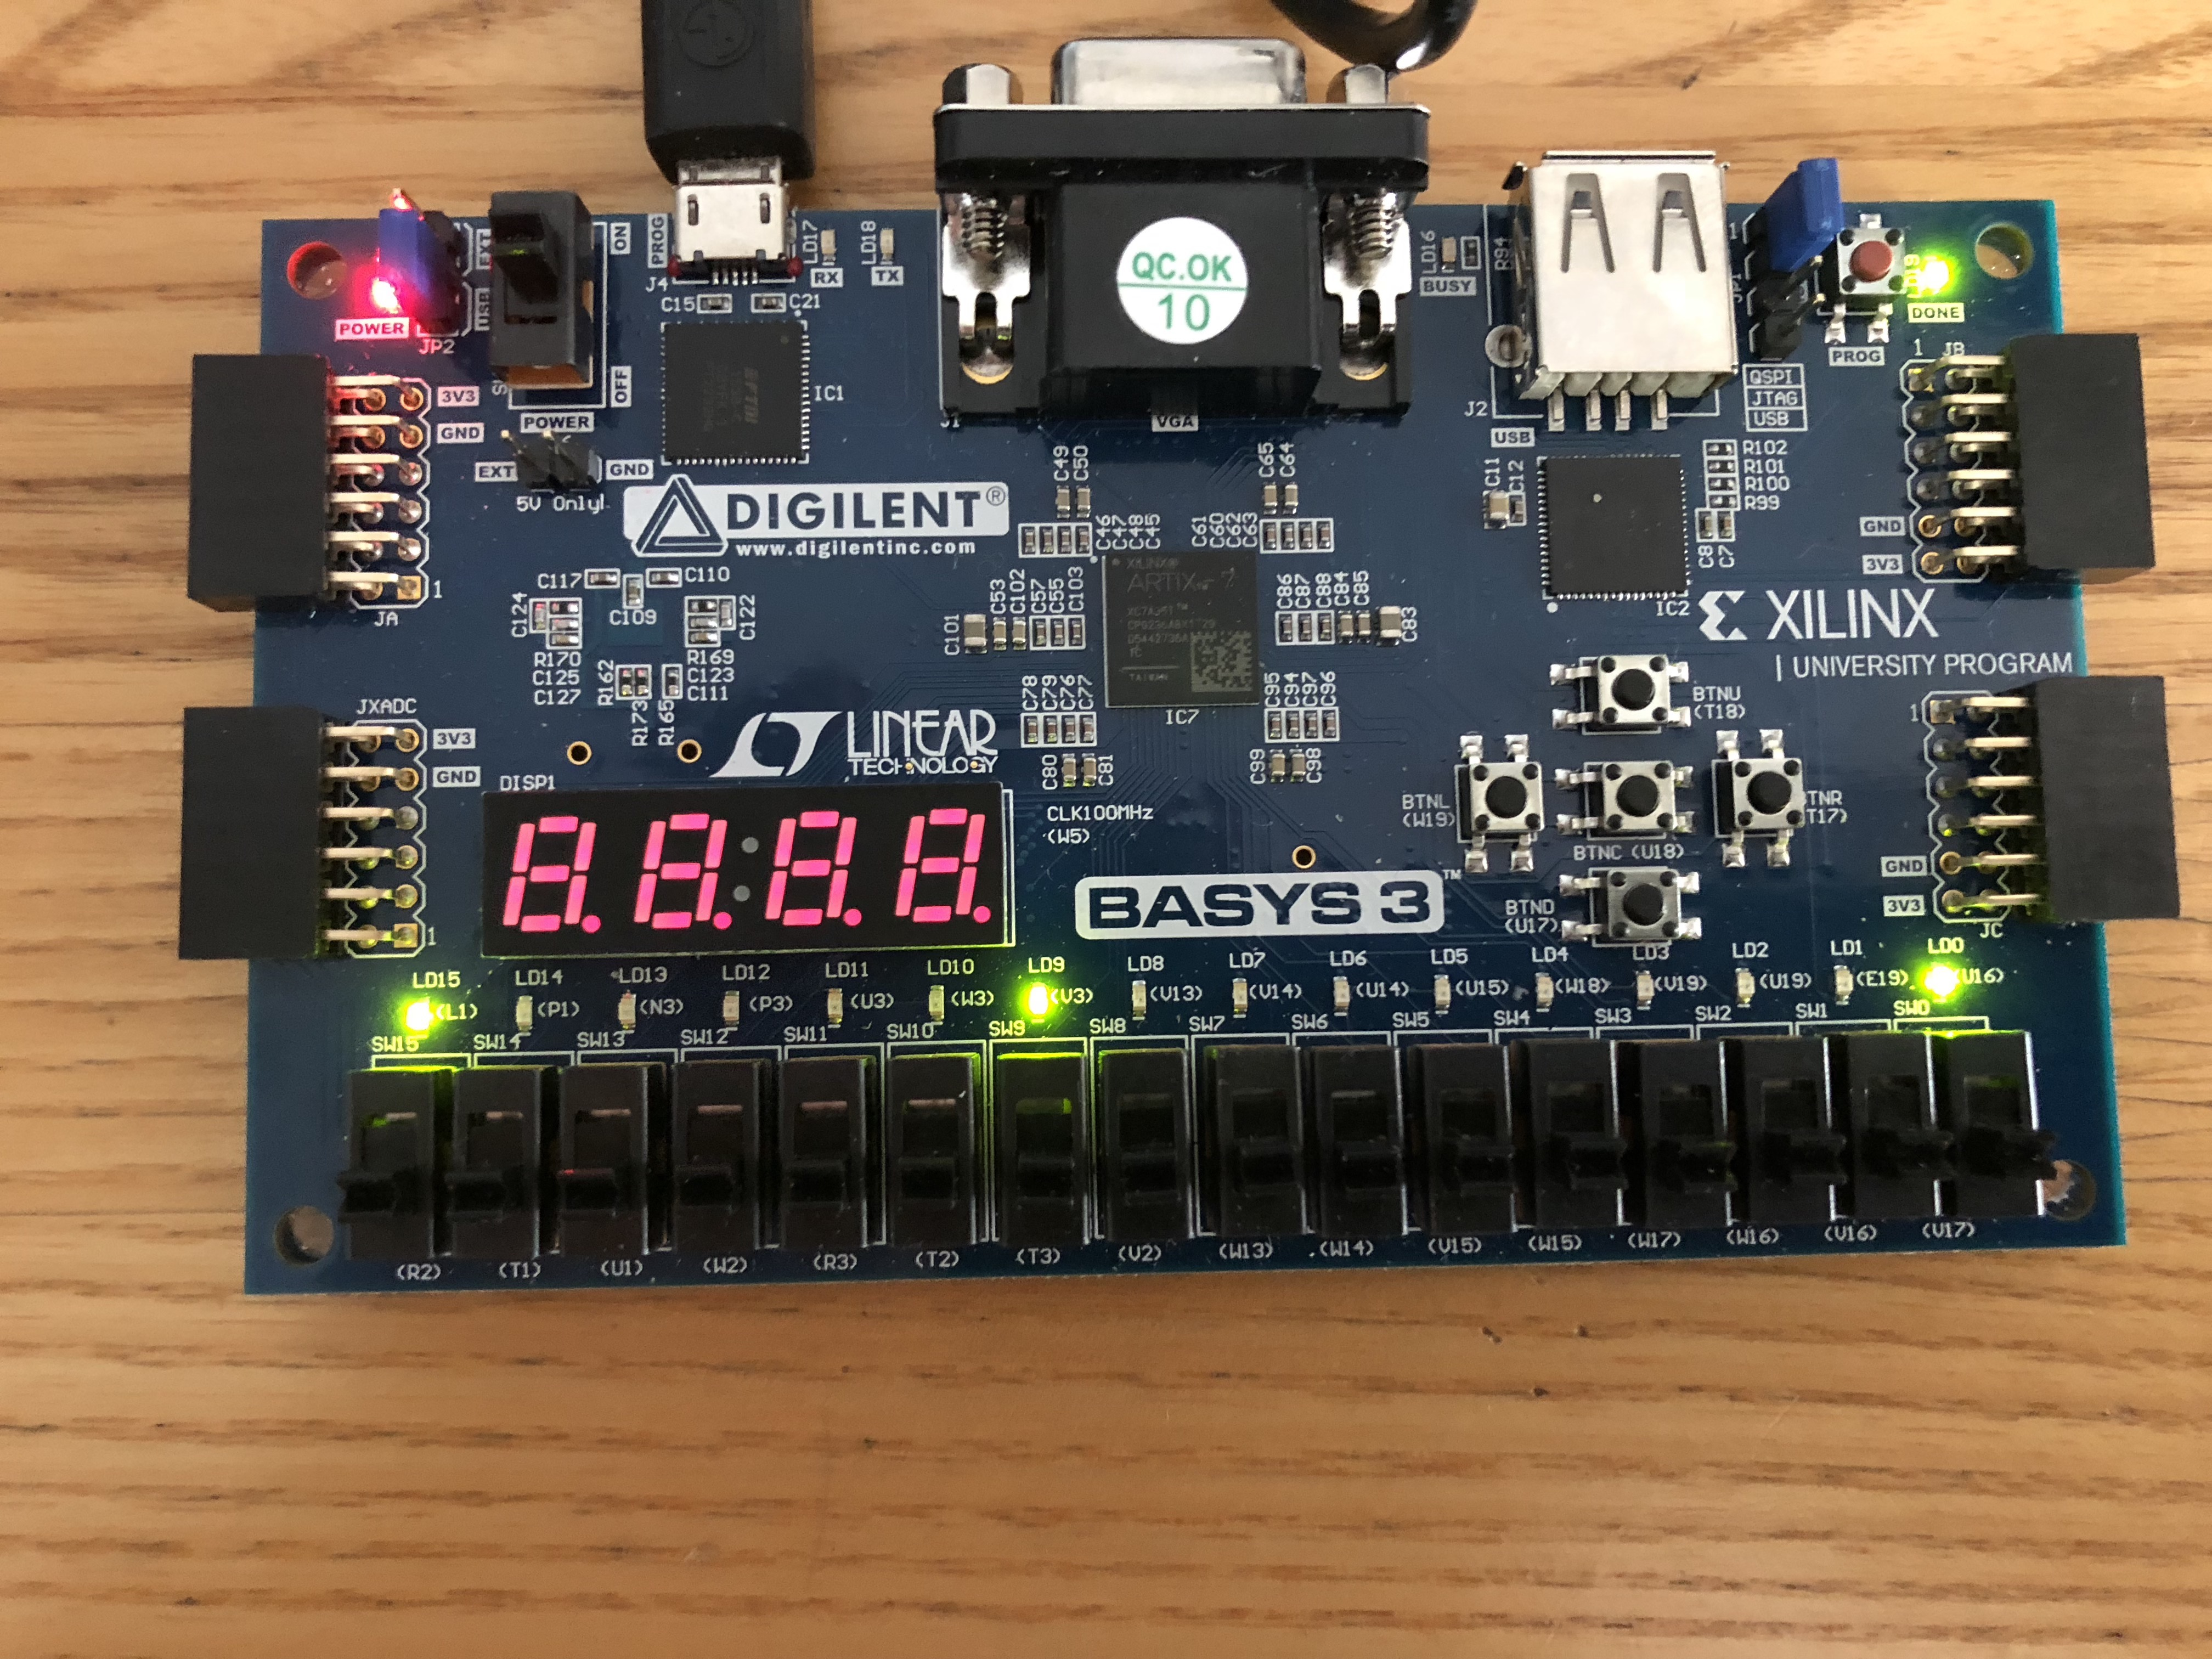
\includegraphics[width=0.5\textwidth]{./images/Part2/l9p2img1.jpg}
	\caption{\label{fig:part2_img1}North and South are green, East/West is red.}
\end{center}
\end{figure}

\begin{figure}[H]
\begin{center}
	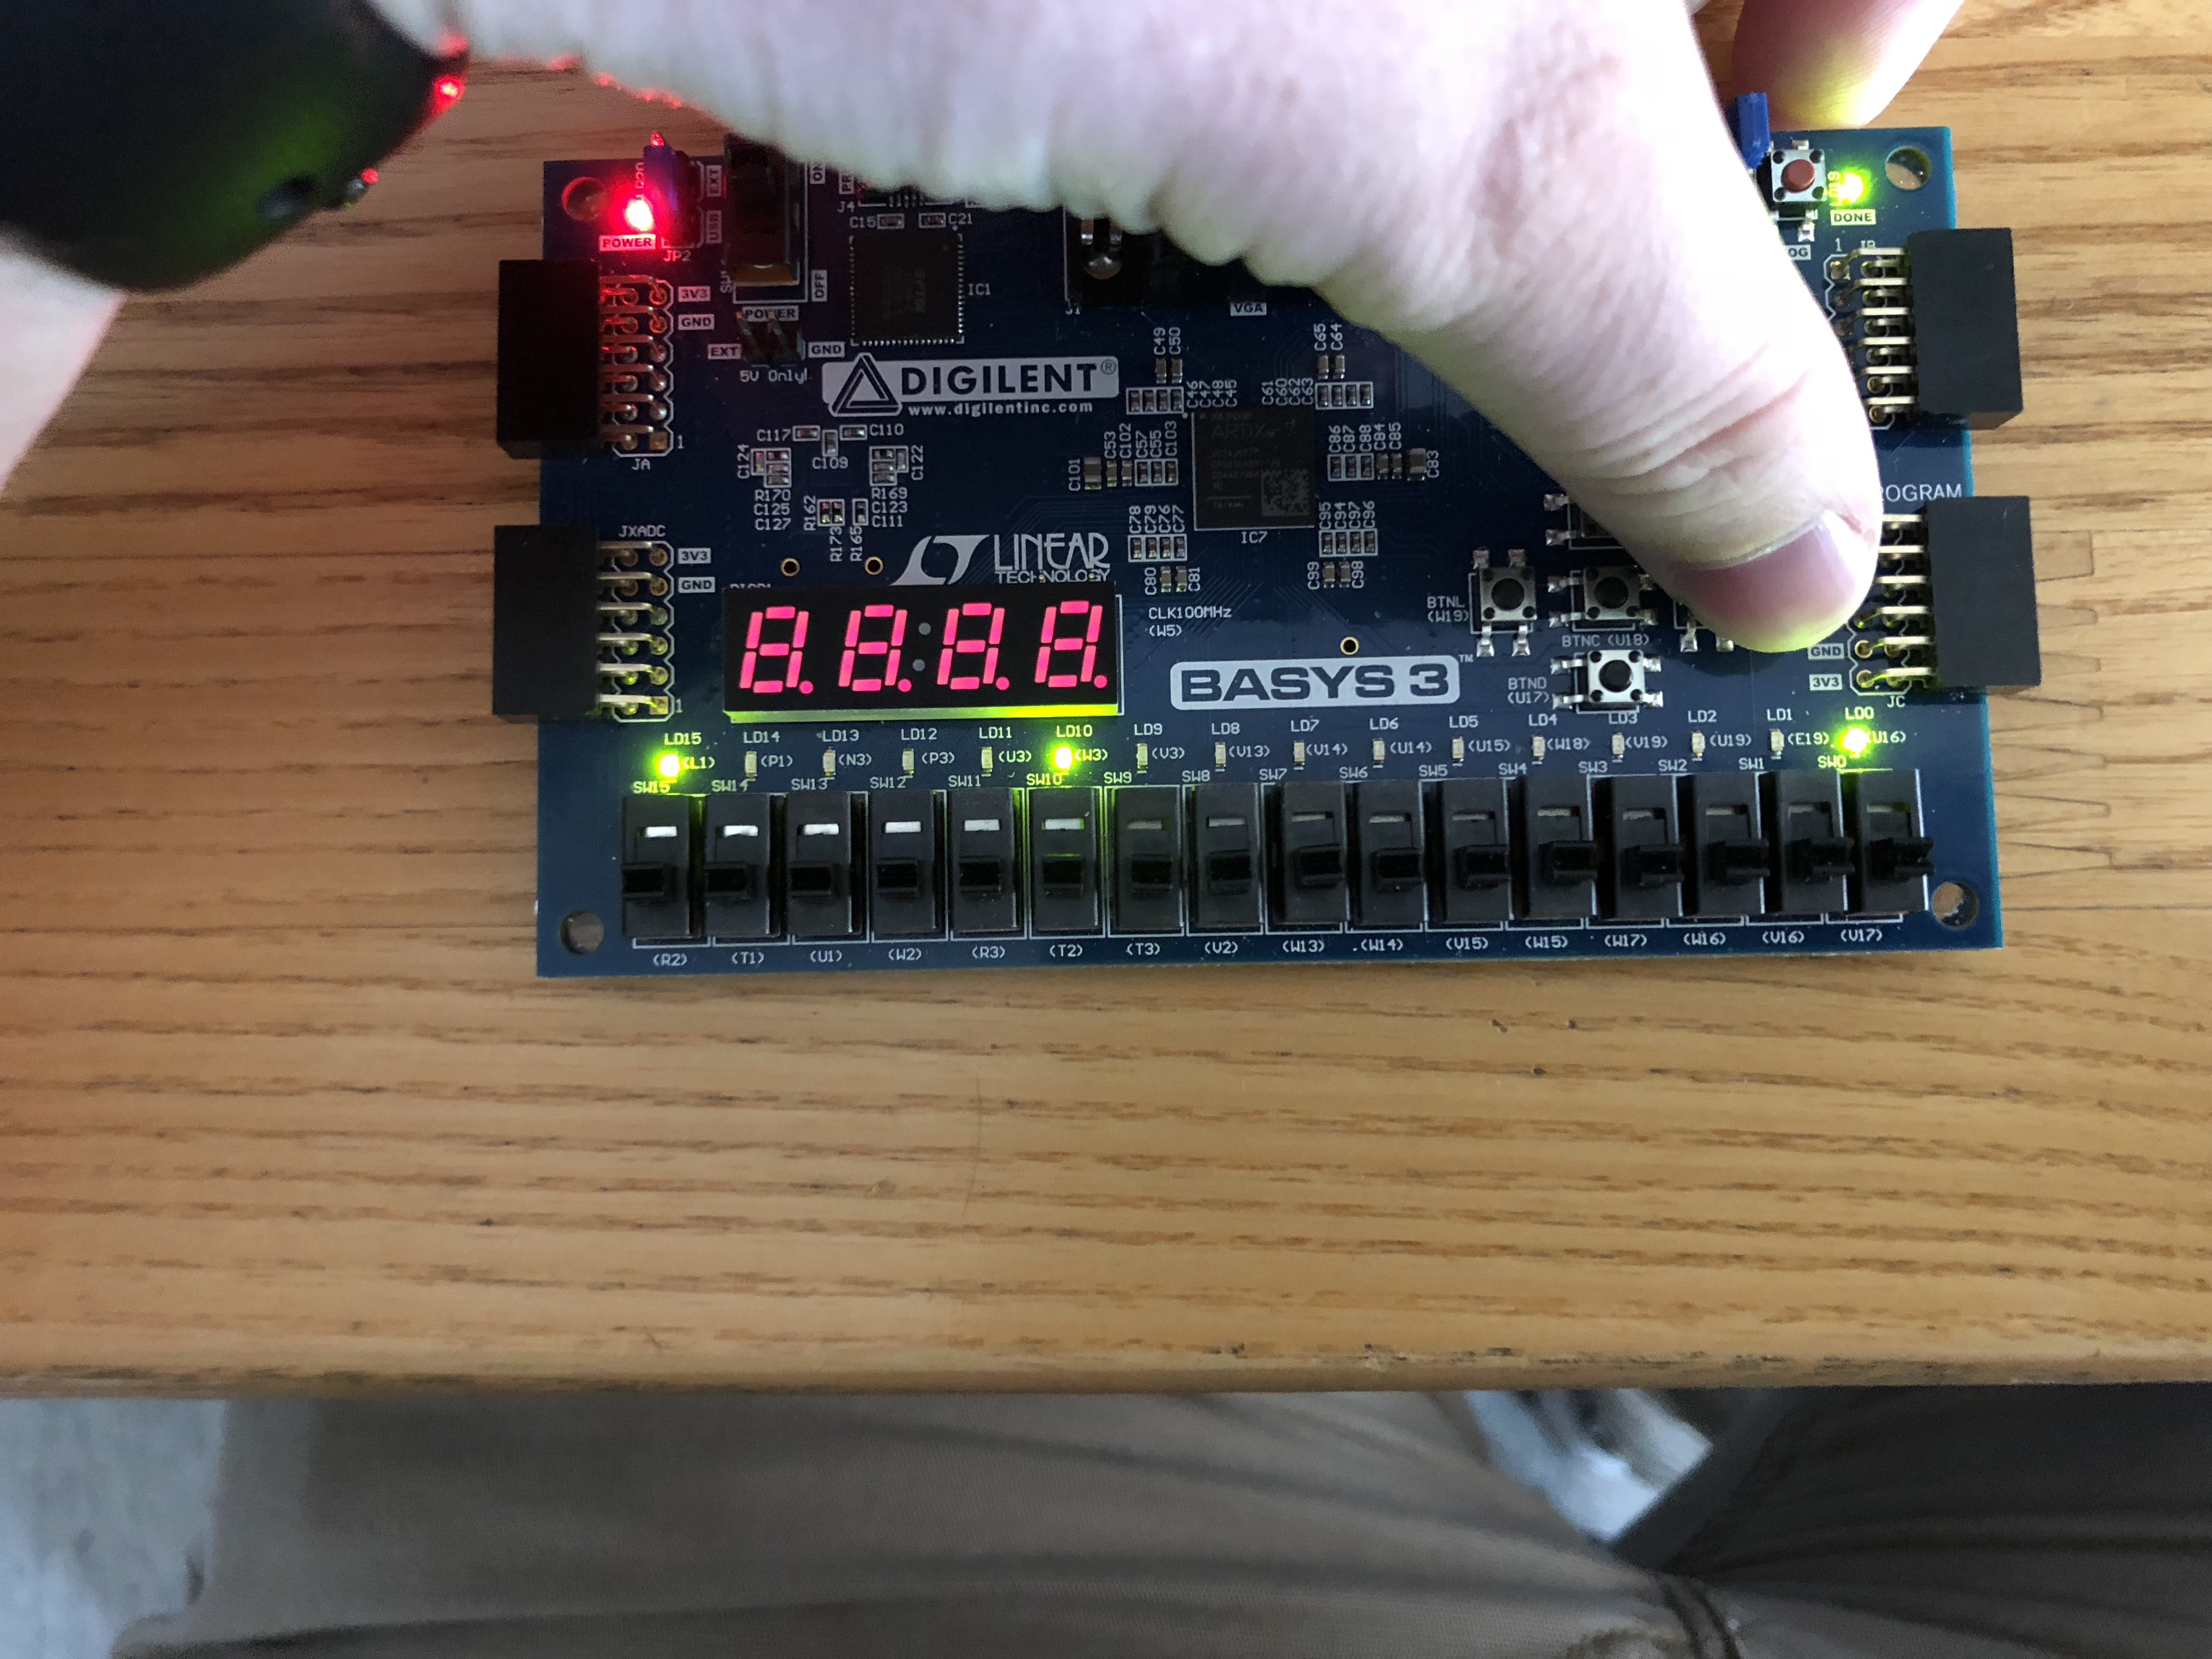
\includegraphics[width=0.5\textwidth]{./images/Part2/l9p2img2.jpg}
	\caption{\label{fig:part2_img2}North Turn sensor is pressed, South turns yellow.}
\end{center}
\end{figure}

\begin{figure}[H]
\begin{center}
	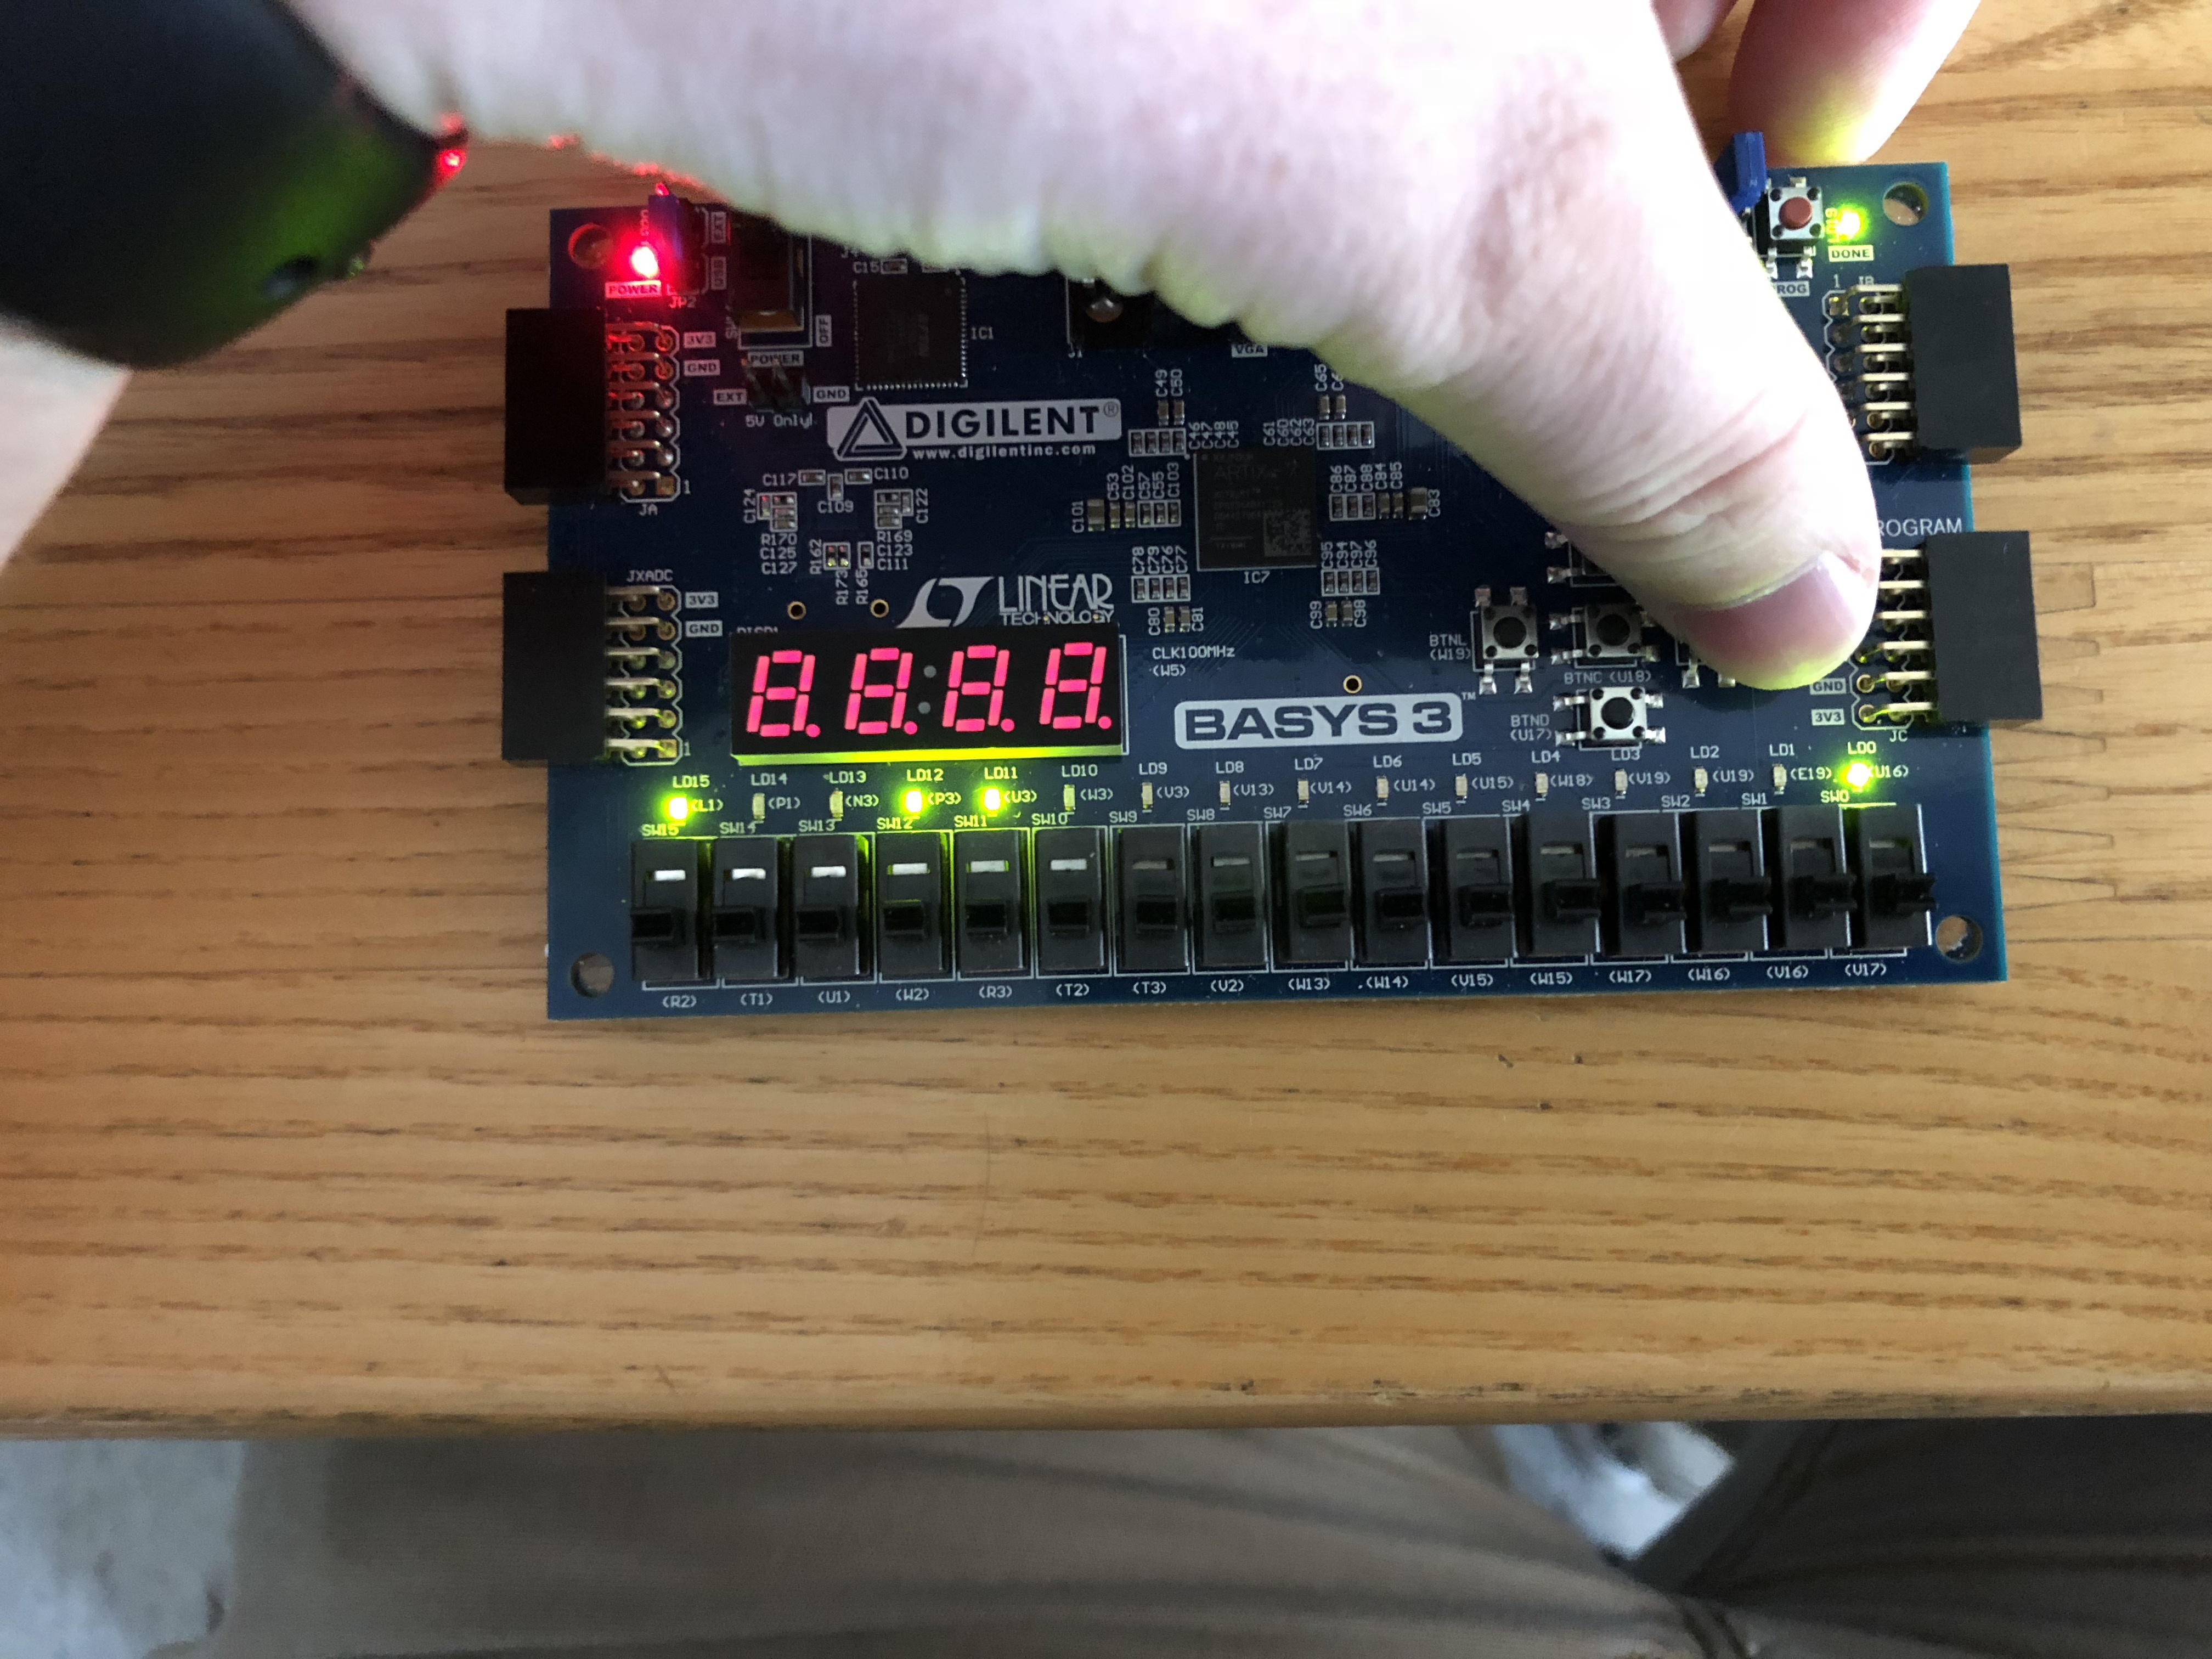
\includegraphics[width=0.5\textwidth]{./images/Part2/l9p2img3.jpg}
	\caption{\label{fig:part2_img3}South turns red for one cycle before turning begins.}
\end{center}
\end{figure}

\begin{figure}[H]
\begin{center}
	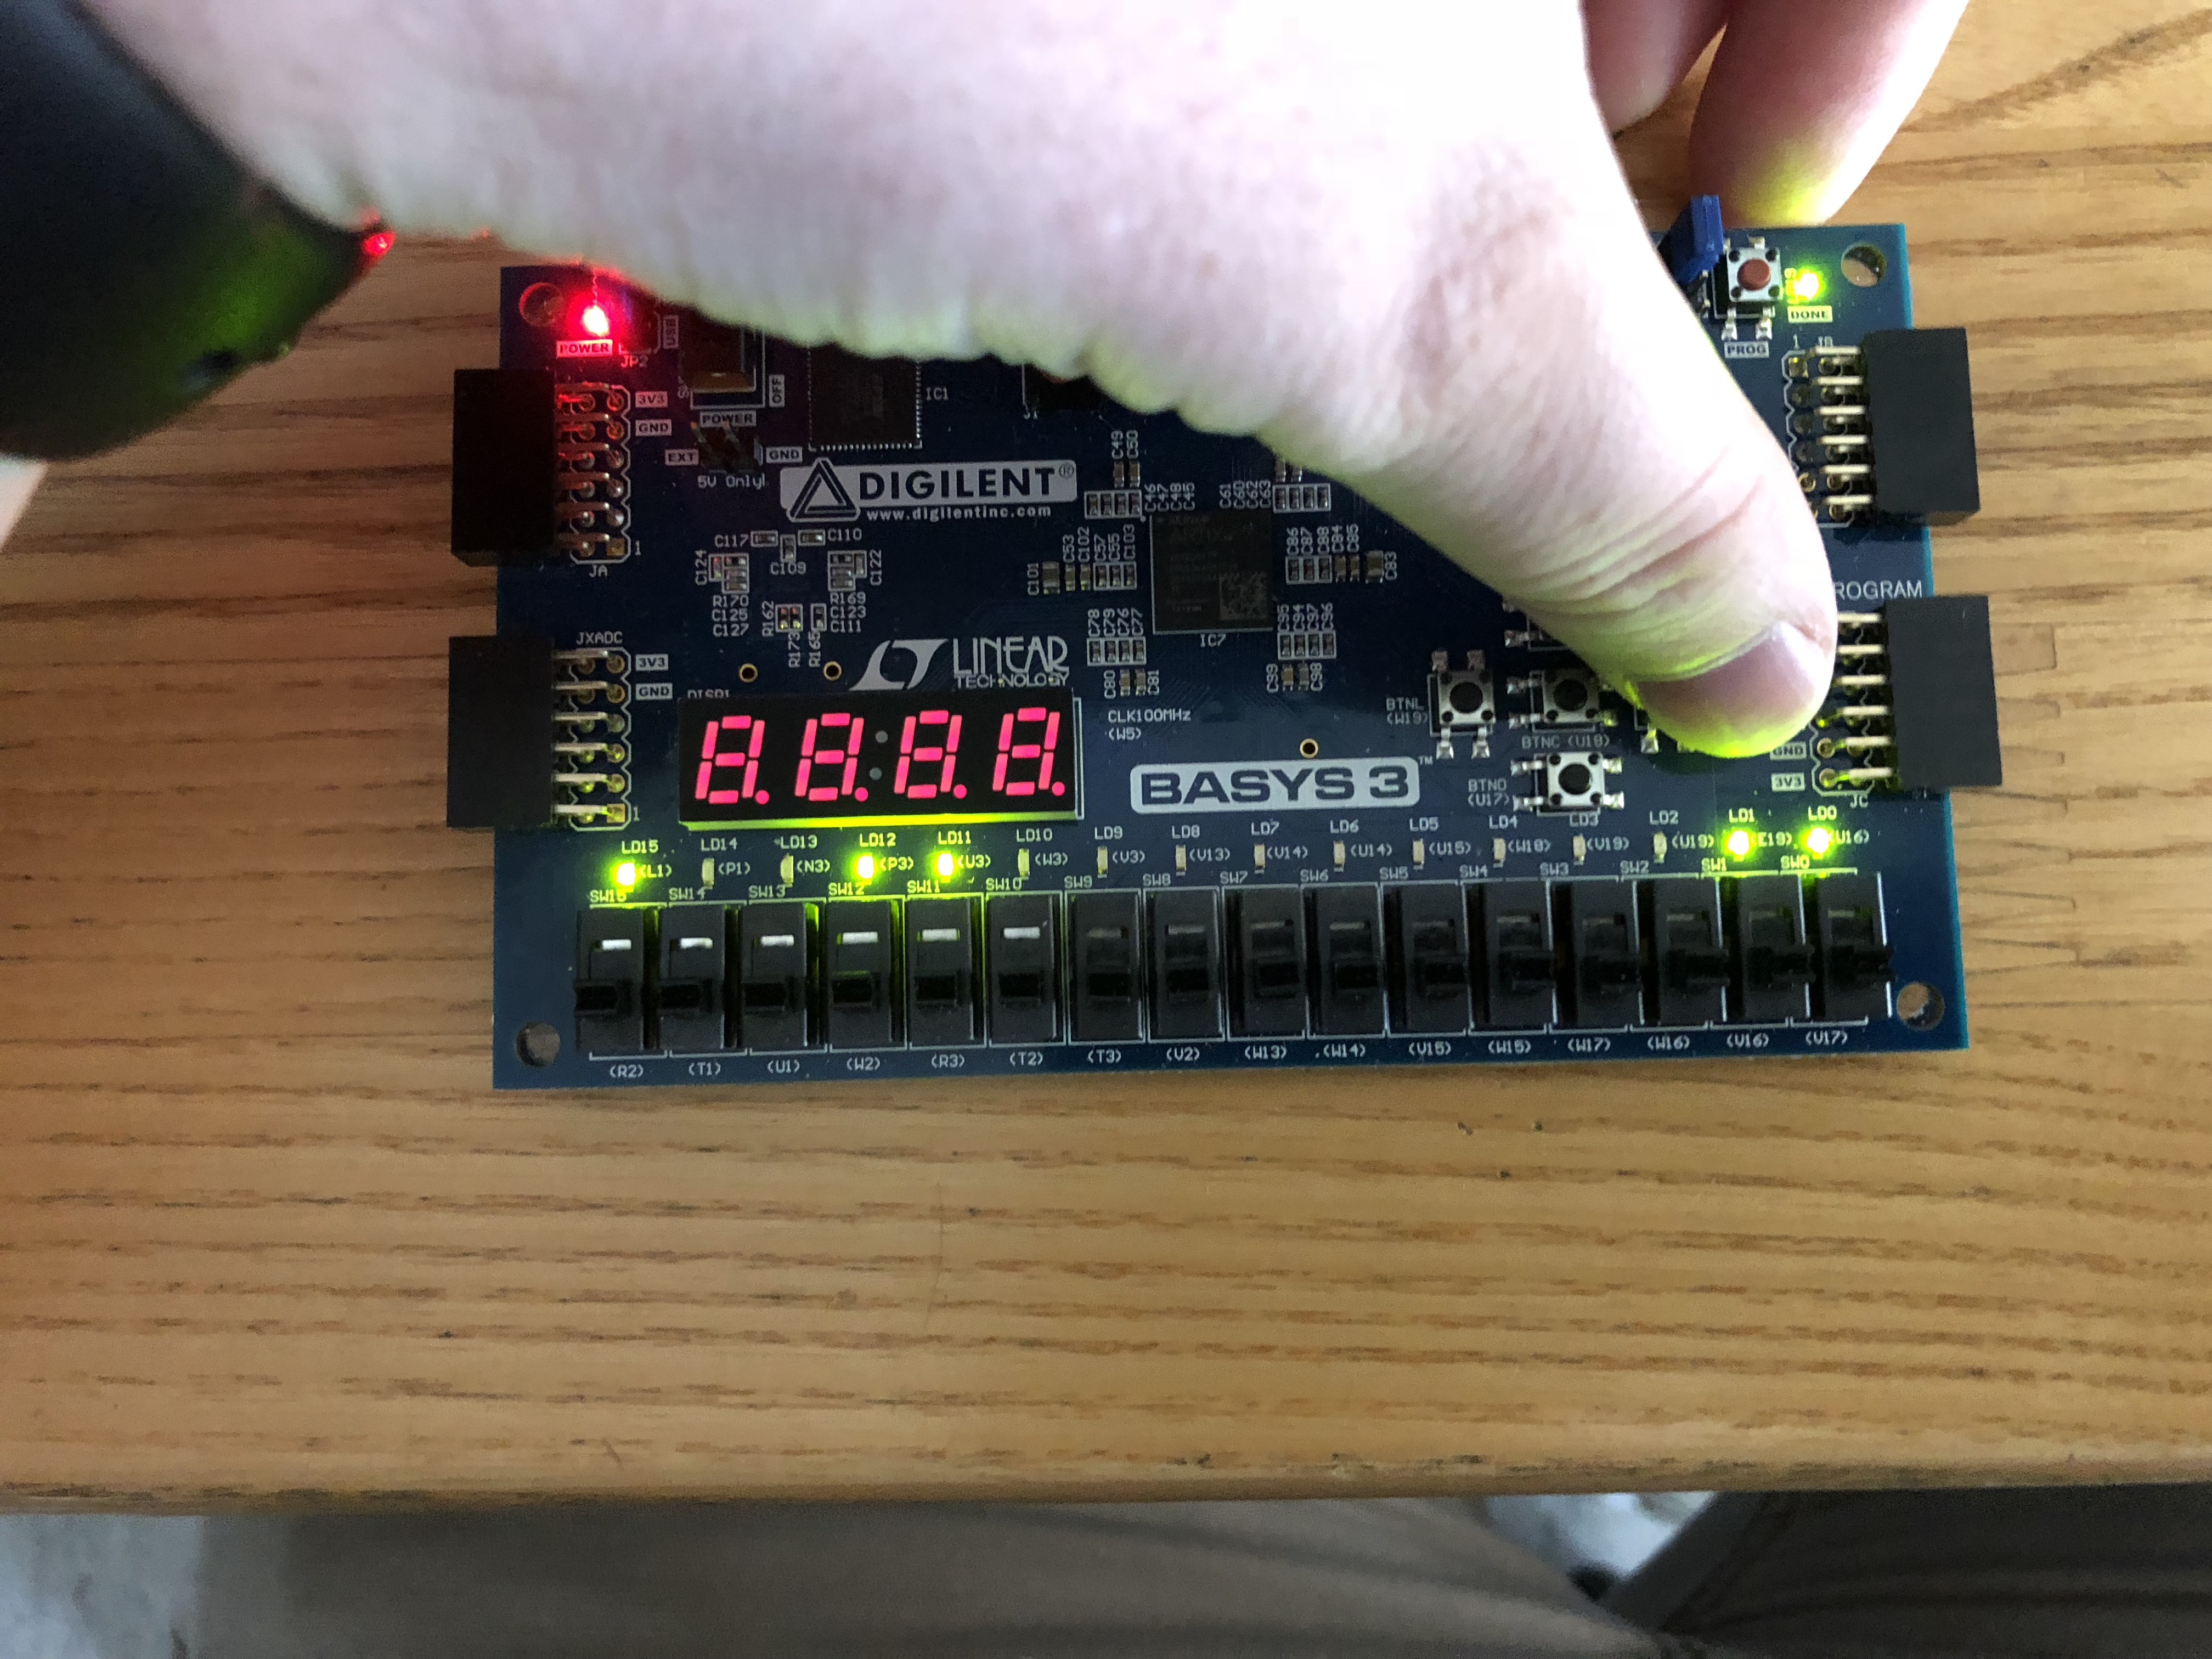
\includegraphics[width=0.5\textwidth]{./images/Part2/l9p2img4.jpg}
	\caption{\label{fig:part2_img4}North turn is green, north remains green. South and East/West are red.}
\end{center}
\end{figure}

\begin{figure}[H]
\begin{center}
	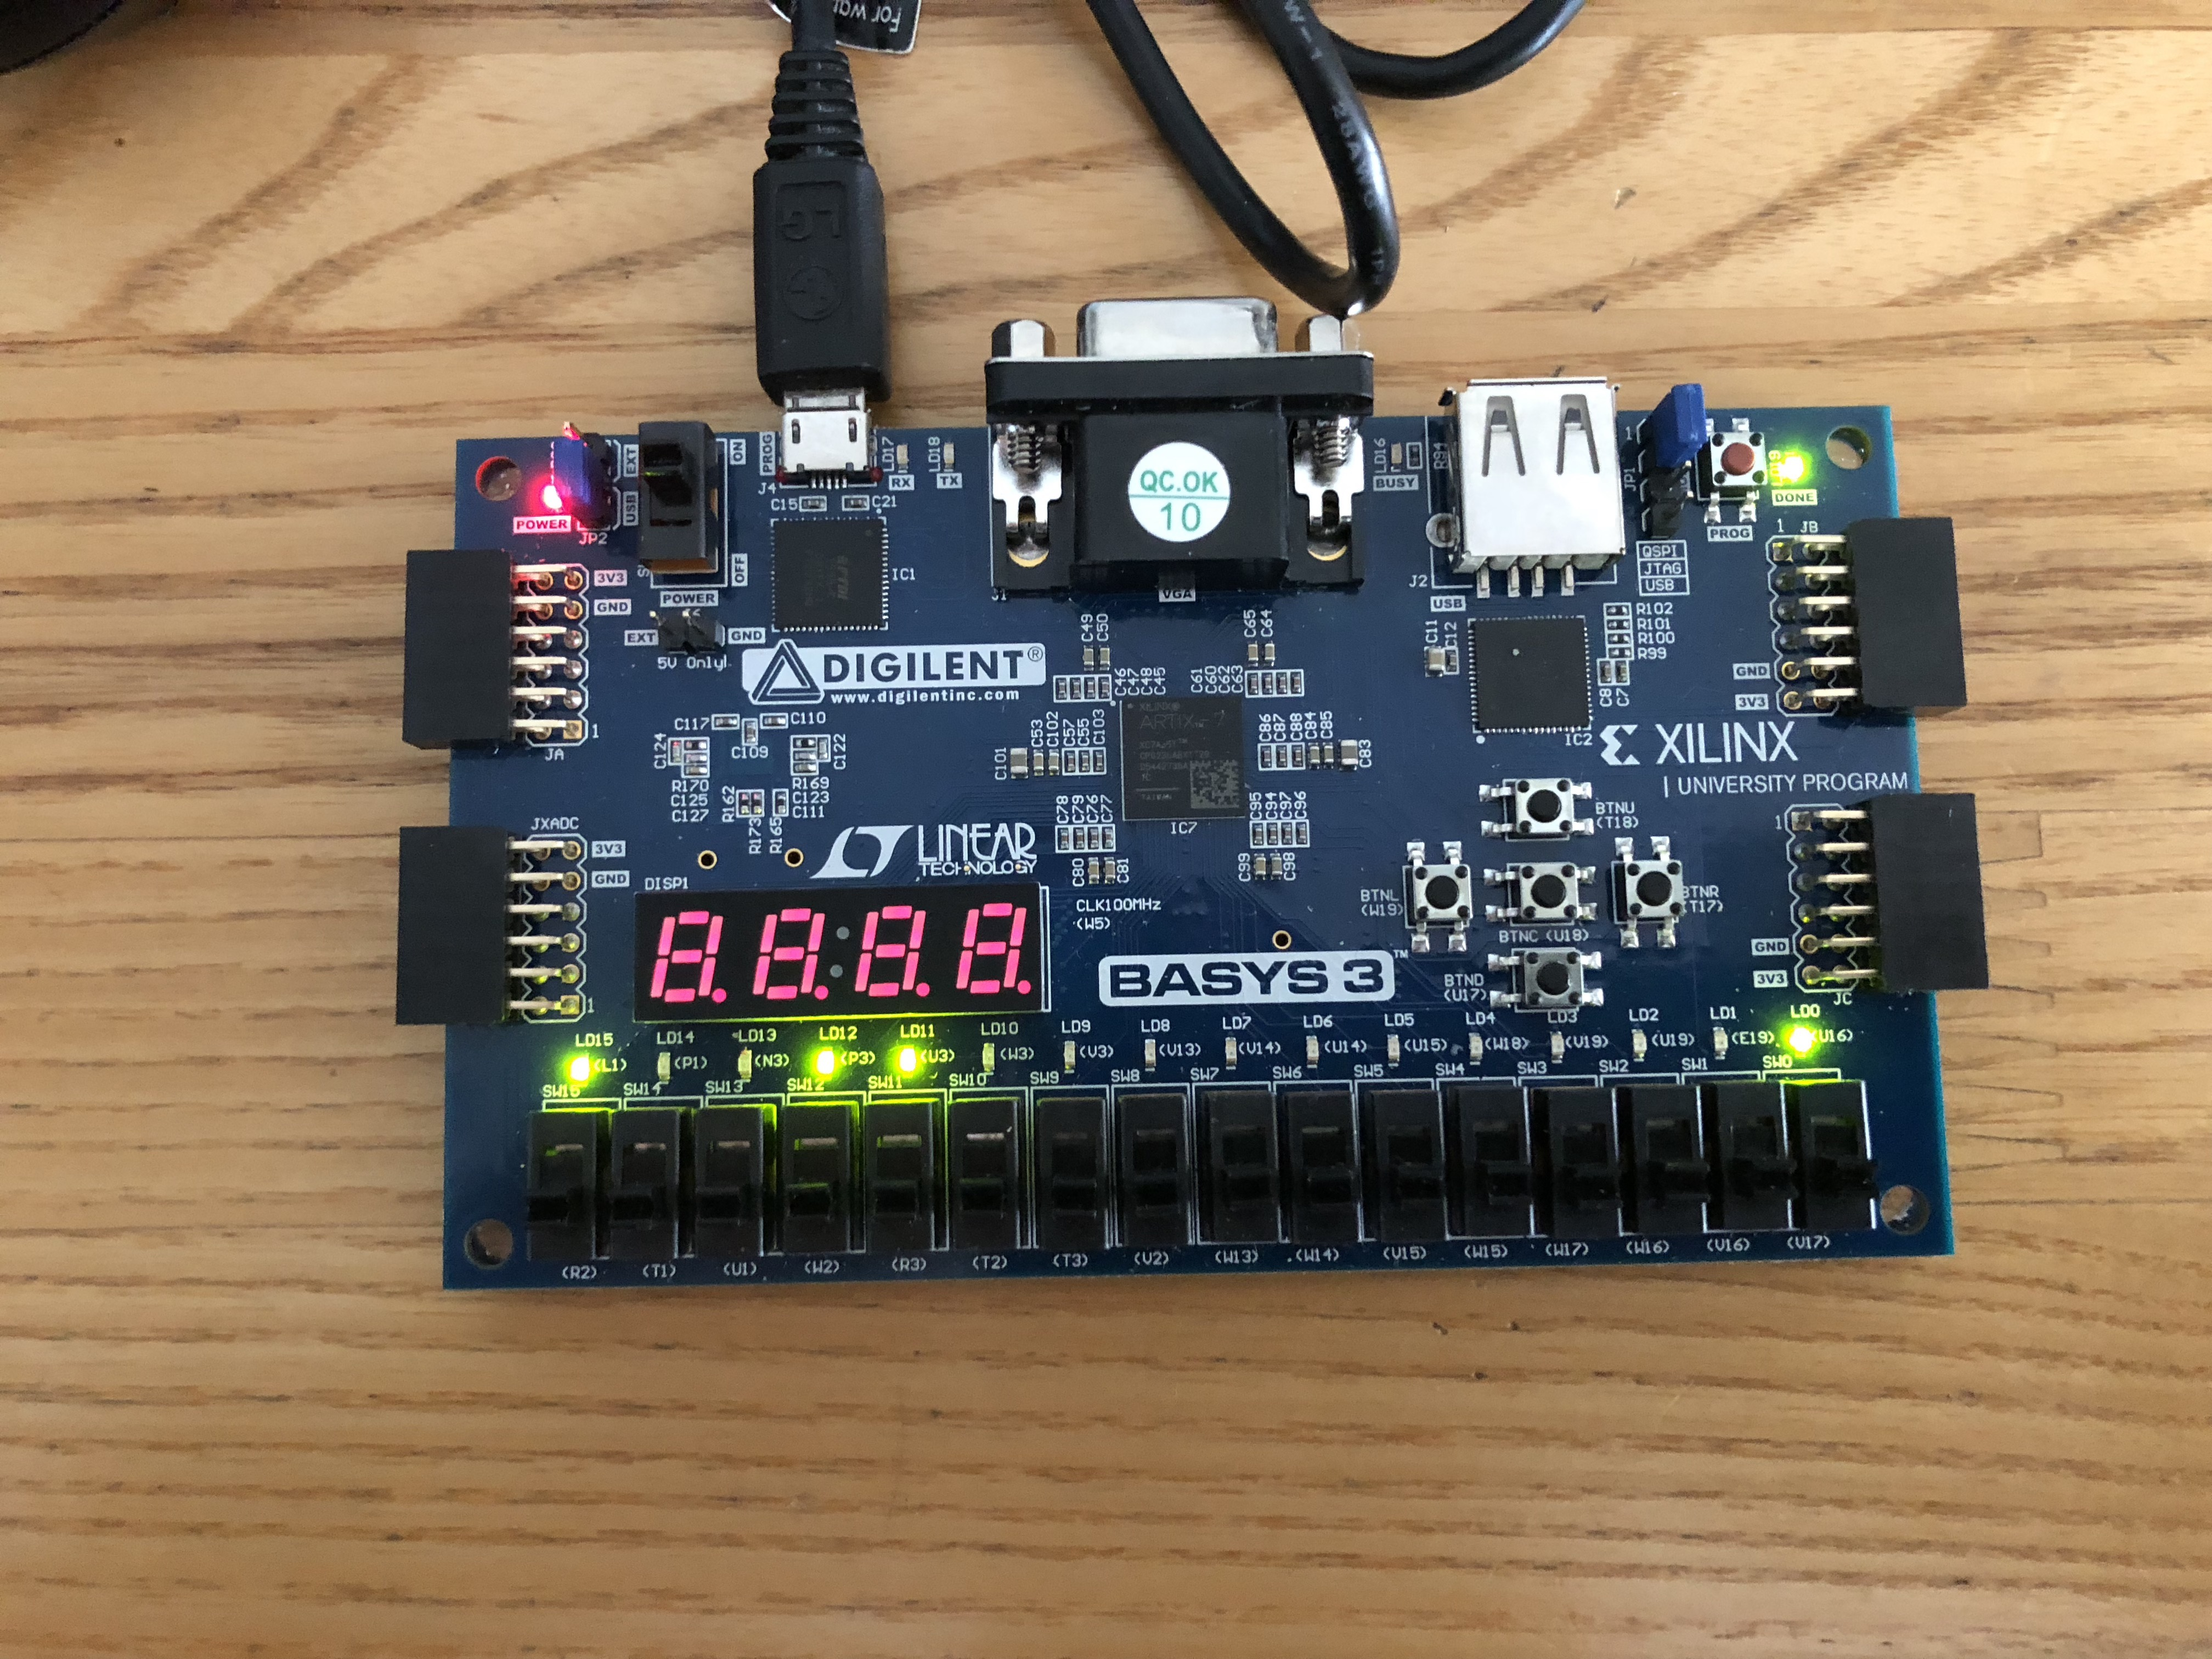
\includegraphics[width=0.5\textwidth]{./images/Part2/l9p2img5.jpg}
	\caption{\label{fig:part2_img5}When North turn sensor is released, North turn is yellow.}
\end{center}
\end{figure}

\begin{figure}[H]
\begin{center}
	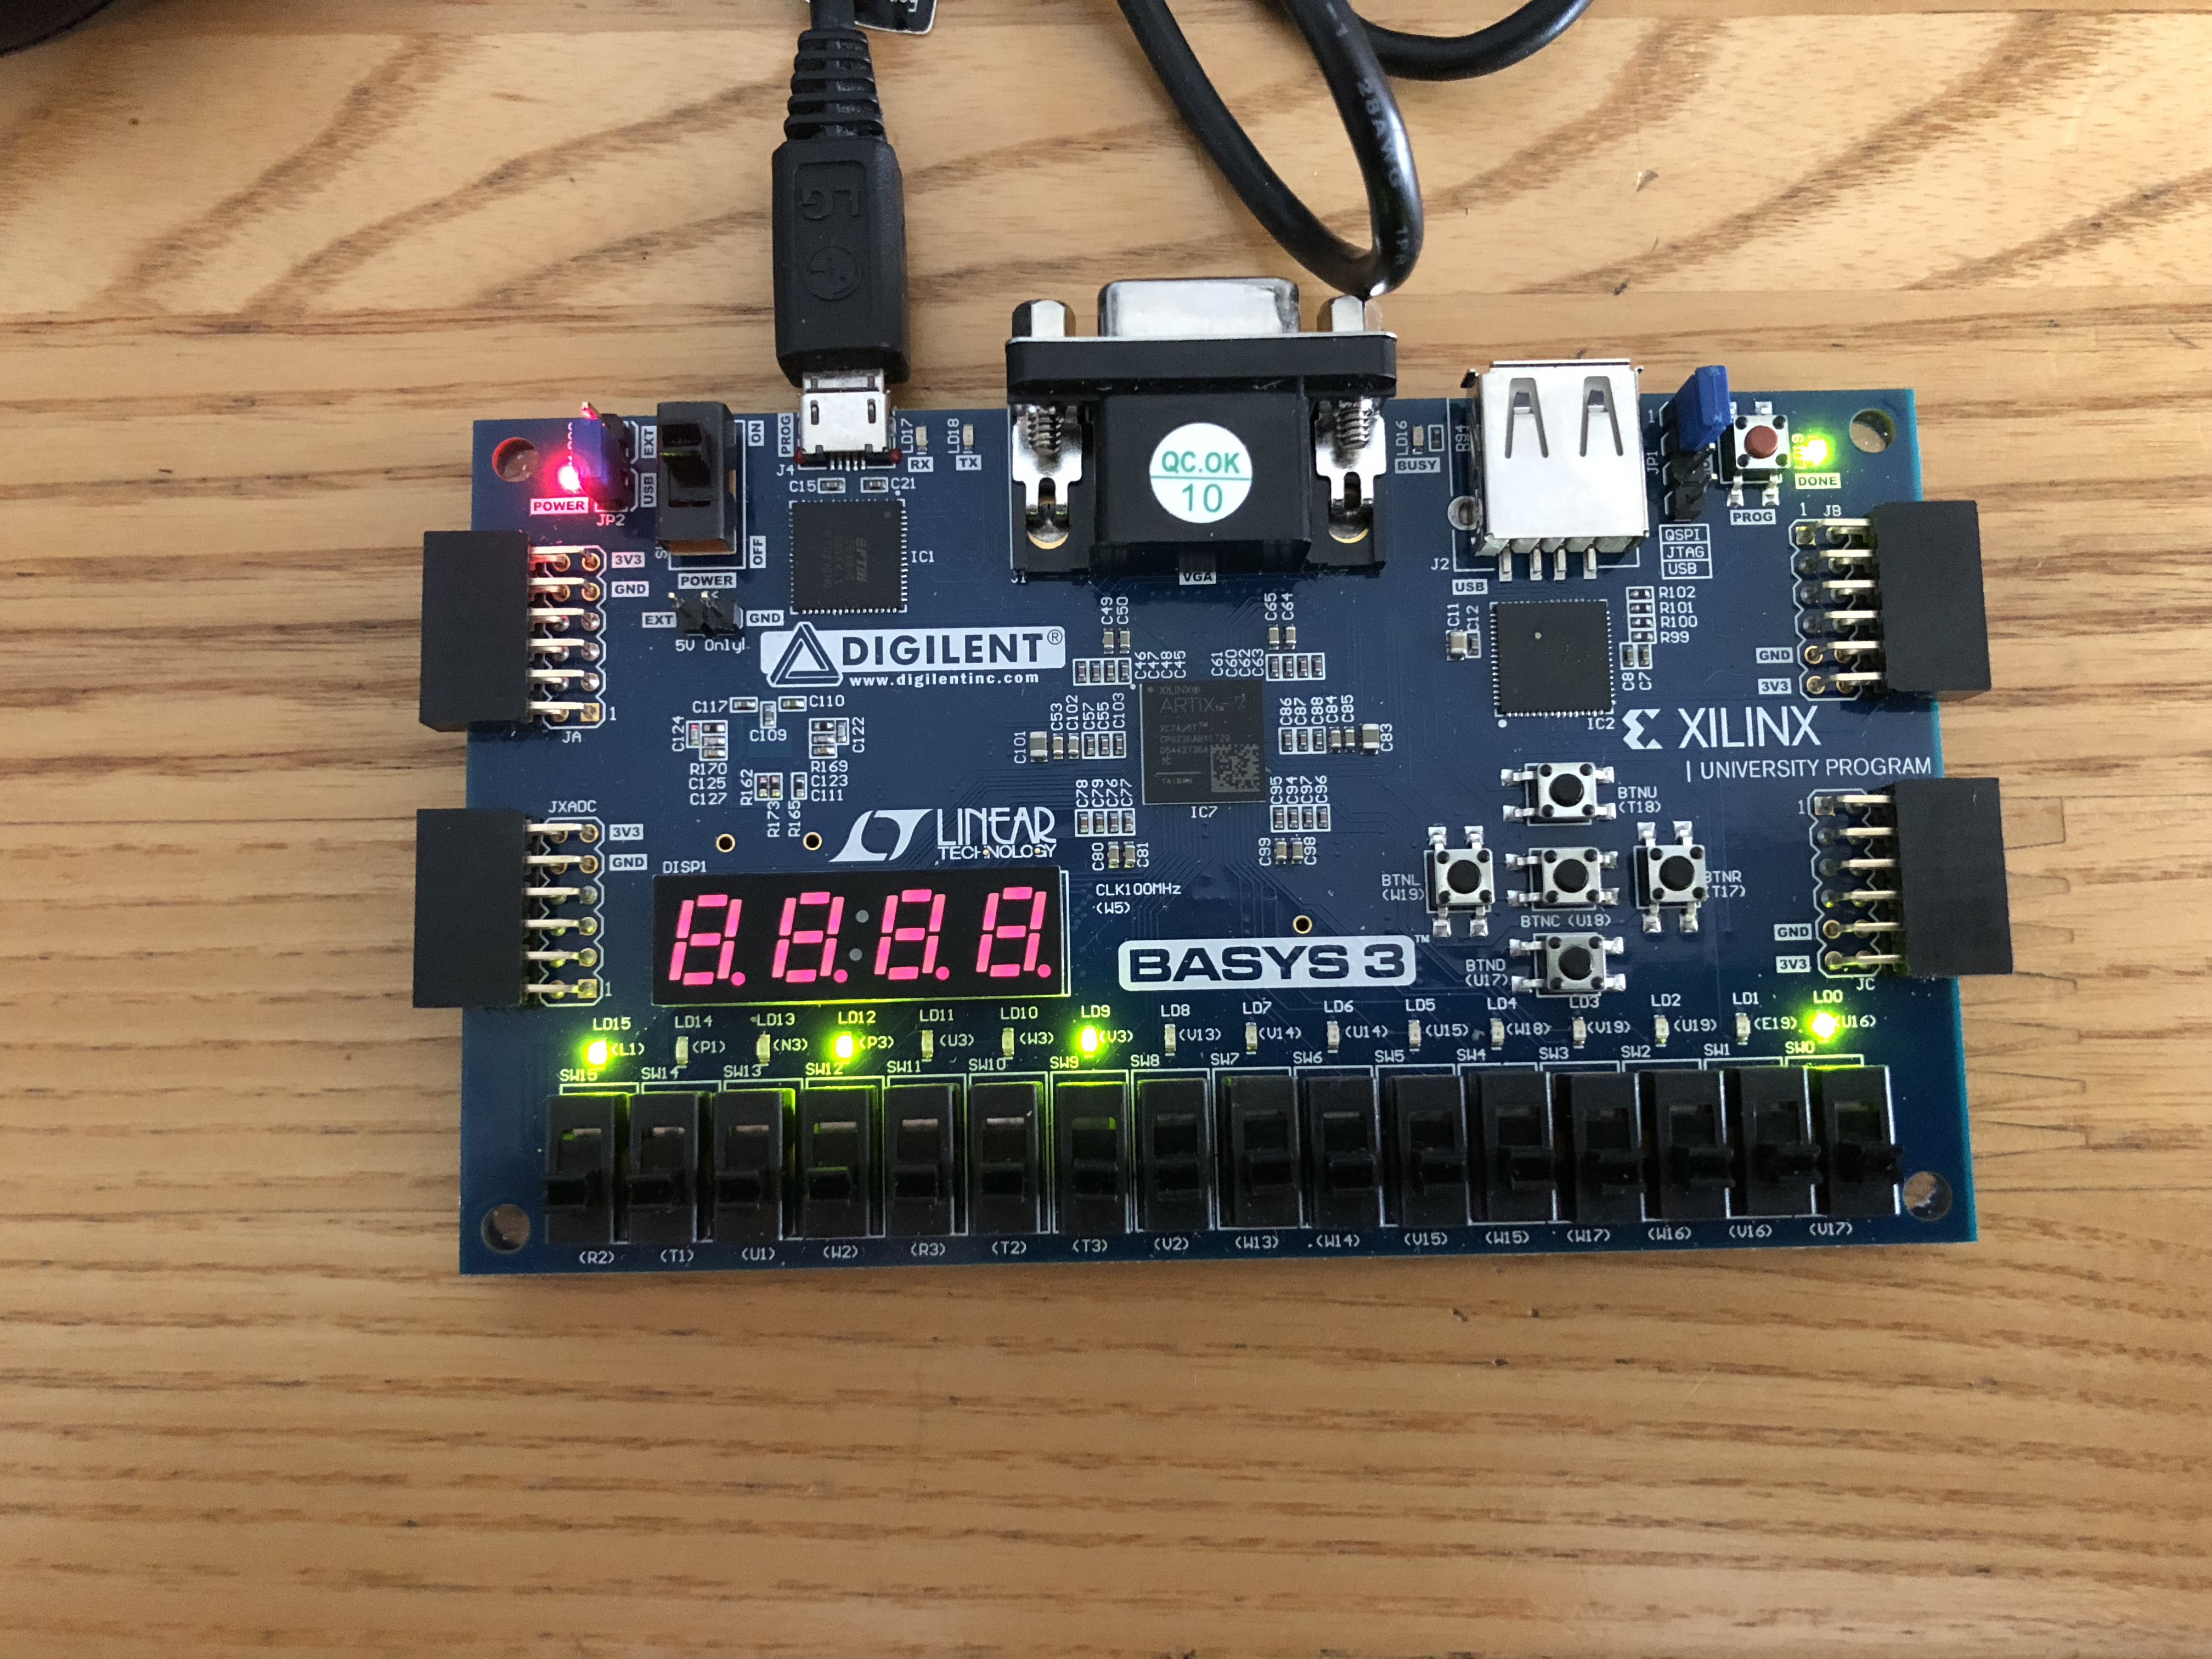
\includegraphics[width=0.5\textwidth]{./images/Part2/l9p2img6.jpg}
	\caption{\label{fig:part2_img6}North turn is totally off for one cycle before south turns green and we return to default state.}
\end{center}
\end{figure}

\subsection{Problem 3}

\subsubsection{Background}
For this problem, we were to keep the same state machine as Problem 2, shown in Figure ~\ref{fig:part2_state_machine}, but add a counter that would count each time the East/West or the North turn sensors were triggered.

\subsubsection{Design Solution}
We implemented an additional entity that will handle the counting when triggered by the sensors. This encapsulation made the overall design easier to manipulate and update. The input ports are defined in Table ~\ref{tab:part3_input_ports} and the outputs are defined in Table ~\ref{tab:part3_output_ports}.

\begin{table}[H]
\begin{center}
\begin{tabular}{| l | l | l |}
	\hline
	Bit & Label & Port \\ \hline
	clk &  Clock & W5 \\ \hline
	reset & Button Center & U18 \\ \hline
	 sensor EW 1 Swtch 0 & & V17 \\ \hline
	sensor EW 0 & Switch 1 & V16 \\ \hline
	sensor NT & Button Right& T17 \\ \hline
\end{tabular}
\caption{\label{tab:part3_input_ports}Input port assignments for  the final traffic system with counters.}
\end{center}
\end{table}

\begin{table}[H]
\begin{center}
\begin{tabular}{| l | l | l |}
	\hline
	Bit & Label & Port \\ \hline
	clk led & LED 12 & P3 \\ \hline
	east west 2 & LED 15 & L1 \\ \hline
	east west 1 & LED 14 & P1 \\ \hline
	east west 0 & LED 13 & N3 \\ \hline
	south 2 & LED 11 & U3 \\ \hline
	south 1 & LED 10 & W3 \\ \hline
	south 0 & LED 9 & V3 \\ \hline
	north 4 & LED 4 & W18 \\ \hline
	north 3 & LED 3 & V19 \\ \hline
	north 2 & LED 2 & U19 \\ \hline
	north 1 & LED 1 & E19 \\ \hline
	north 0 & LED 0 & U16 \\ \hline
	output count 6 & CA & W7 \\ \hline
	output count 5 & CB & W6 \\ \hline
	output count 4 & CC & U8 \\ \hline
	output count 3 & CD & V8 \\ \hline
	output count 2 & CE & U5 \\ \hline
	output count 1 & CF & V5 \\ \hline
	output count 0 & CG & U7 \\ \hline
	output mux 3 & AN3 & W4 \\ \hline
	output mux 2 & AN2 & V4 \\ \hline
	output mux 1 & AN1 & U4 \\ \hline
	output mux 0 & AN0 & U2 \\ \hline
\end{tabular}
\caption{\label{tab:part3_output_ports}Output port assignments for the final traffic system with counters.}
\end{center}
\end{table}

\subsubsection{Results}
We were unable to successfully implement this design on the board. Our counters appeared to work properly, but we were unable to display this data using the seven segment displays. The most difficult challenge for this portion was trying to figure out the display driver signal that would show different outputs using seven-segment digits.

\section{Conclusion}
This lab was an excellent example of a real world problem that we can design a solution for based on our skills learned in this class. It was very challenging to receive a trigger from a signal that isn't a clock, as well as to output different signals to seven segment displays.

\pagebreak

\textbf{Appendices}

\begin{appendices}

\section{Clock Divider VHDL Code}
This code for a clock divider is used in each part of the lab.

\begin{lstlisting}[language=VHDL]
library IEEE;
use IEEE.STD_LOGIC_1164.ALL;
use IEEE.NUMERIC_STD.ALL;

entity Clockdivider is
     port(clk : in std_logic;
          start_timer : in std_logic;
	  FastClock,MediumClock,SlowClock, led0 : out std_logic);
end Clockdivider;

architecture clockdivider_arch of Clockdivider is
signal slowClock_sig : STD_LOGIC;
begin
    process  
    variable cnt :	std_logic_vector(26 downto 0):=
     "000000000000000000000000000";
    begin					 
        wait until ((clk'EVENT) AND (clk = '1'));
		if (start_timer = '1') then
	       cnt := "000000000000000000000000000";
	    else  
           cnt := STD_LOGIC_VECTOR(unsigned(cnt) + 1);
	    end if;
   	    FastClock <= cnt(22);
   	    MediumClock <= cnt(24);	
   	    SlowClock <= cnt(26);
        slowClock_sig <= cnt(26);
        if (slowClock_sig = '1') then
		  led0 <= '1';
	    else
		  led0 <= '0';
	    end if;
	end process;
end clockdivider_arch;
\end{lstlisting}

\section{Problem 1 VHDL Code}

\begin{lstlisting}[language=VHDL]
library IEEE;
use IEEE.STD_LOGIC_1164.ALL;

entity Lab9Part1 is
    Port ( clk : in STD_LOGIC;
           reset : in STD_LOGIC;
           sensors_EW : in STD_LOGIC;
           north : out STD_LOGIC_VECTOR(4 downto 0);
           south : out STD_LOGIC_VECTOR(2 downto 0);
           east_west : out STD_LOGIC_VECTOR(2 downto 0);
           clock_led : out STD_LOGIC);
end Lab9Part1;

architecture Behavioral of Lab9Part1 is

component Clockdivider is
     port(clk : in std_logic;
          start_timer : in std_logic;
	  FastClock,MediumClock,SlowClock, led0 : out std_logic);
end component Clockdivider;

signal current_state : STD_LOGIC_VECTOR(3 downto 0) := "0000";
signal next_state : STD_LOGIC_VECTOR(3 downto 0) := "0000";
signal start_timer : STD_LOGIC := '0';
signal fast_clock : STD_LOGIC;
signal medium_clock : STD_LOGIC;
signal slow_clock : STD_LOGIC;

begin
    clk_div : ClockDivider port map(clk, start_timer, fast_clock,
     medium_clock, slow_clock, clock_led);
    
    process(slow_clock, reset)
    begin
        if(reset = '1') then next_state <= "0000";
        elsif(slow_clock'event and slow_clock = '1') then
            case current_state is
                when "0000" =>
                    next_state <= "0001";
                when "0001" =>
                    next_state <= "0010";
                when "0010" =>
                    next_state <= "0011";
                when "0011" =>
                    next_state <= "0100";
                when "0100" =>
                    next_state <= "0101";
                when "0101" =>
                    next_state <= "0110";
                when "0110" =>
                    next_state <= "0111";
                when "0111" =>
                    next_state <= "1000";
                when others =>
                    next_state <= "0000";
            end case;
        end if;
    end process;
    process(current_state)
    begin
        case current_state is
            when "0000" =>
                north <= "00001";
                south <= "001";
                east_west <= "100";
            when "0001" =>
                north <= "01000";
                south <= "010";
                east_west <= "100";
            when "0010" =>
                north <= "10000";
                south <= "100";
                east_west <= "100";
            when "0011" =>
                north <= "10000";
                south <= "100";
                east_west <= "001";
            when "0100" =>
                north <= "10000";
                south <= "100";
                east_west <= "010";
            when "0101" =>
                north <= "10000";
                south <= "100";
                east_west <= "100";
            when "0110" =>
                north <= "00011";
                south <= "100";
                east_west <= "100";
            when "0111" =>
                north <= "00101";
                south <= "100";
                east_west <= "100";
            when others =>
                north <= "00001";
                south <= "100";
                east_west <= "100";
        end case;
    end process;
    current_state <= next_state;
end Behavioral;
\end{lstlisting}

\section{Problem 1 Constraints File}
\begin{center}
\begin{figure}[H]
	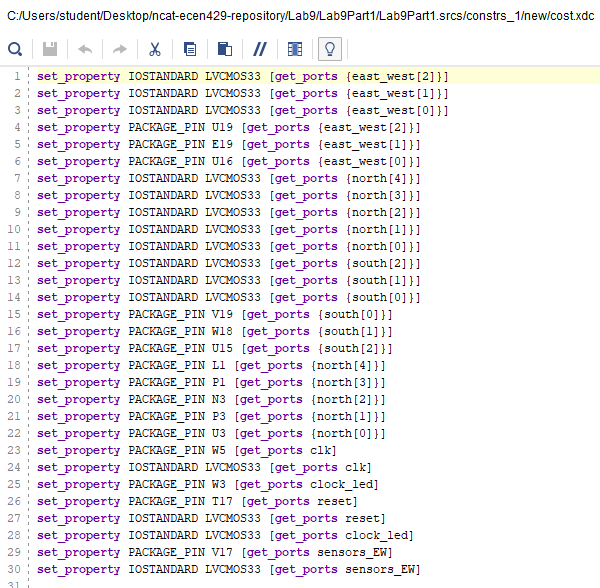
\includegraphics[scale=1]{./images/Part1/l9p1const.png}
	\caption{\label{fig:Prob1Const}Constraints file for Problem 1.}
\end{figure}
\end{center}

\section{Problem 2 VHDL Code}
\begin{lstlisting}[language=VHDL]
library IEEE;
use IEEE.STD_LOGIC_1164.ALL;

entity Lab9Part2 is
    Port ( clk : in STD_LOGIC;
           reset : in STD_LOGIC;
           sensors_EW : in STD_LOGIC_VECTOR(1 downto 0);
           sensor_NT : in STD_LOGIC;
           north : out STD_LOGIC_VECTOR(4 downto 0);
           south : out STD_LOGIC_VECTOR(2 downto 0);
           east_west : out STD_LOGIC_VECTOR(2 downto 0);
           clock_led : out STD_LOGIC);
end Lab9Part2;

architecture Behavioral of Lab9Part2 is

component clock_divider is
     port(clk : in std_logic;
          start_timer : in std_logic;
	  FastClock,MediumClock,SlowClock, led0 : out std_logic);
end component clock_divider;

signal current_state : STD_LOGIC_VECTOR(3 downto 0) := "0000";
signal next_state : STD_LOGIC_VECTOR(3 downto 0) := "0000";
signal start_timer : STD_LOGIC := '0';
signal fast_clock : STD_LOGIC;
signal medium_clock : STD_LOGIC;
signal slow_clock : STD_LOGIC;

begin
    clk_div : clock_divider port map(clk, start_timer, fast_clock,
     medium_clock, slow_clock, clock_led);
    
    process(slow_clock, reset)
    begin
        if(reset = '1') then next_state <= "0000";
        elsif(slow_clock'event and slow_clock = '1') then
            case current_state is
                when "0000" =>
                    if(sensors_EW = "01" or sensors_EW = "10" 
                    or sensors_EW = "11") then
                        next_state <= "0001";
                    elsif(sensor_NT = '1') then 
                        next_state <= "0111";
                    else
                        next_state <= "0000";
                    end if;
                when "0001" =>
                    next_state <= "0010";
                when "0010" =>
                    next_state <= "0011";
                when "0011" =>
                    if(sensors_EW = "01" or sensors_EW = "10"
                     or sensors_EW = "11") then
                        next_state <= "0011";
                    else
                        next_state <= "0100";
                    end if;
                when "0100" =>
                    next_state <= "0101";
                when "0101" =>
                    if(sensor_NT = '1') then
                        next_state <= "0110";
                    else
                        next_state <= "0000";
                    end if;
                when "0110" =>
                    if(sensor_NT = '1') then
                        next_state <= "0110";
                    else
                        next_state <= "1001";
                    end if;
                when "0111" =>
                    next_state <= "1000";
                when "1000" =>
                    next_state <= "0110";
                when "1001" =>
                    next_state <= "1010";
                when others =>
                    next_state <= "0000";
            end case;
        end if;
    end process;
    process(current_state)
    begin
        case current_state is
            when "0000" =>
                north <= "00001";
                south <= "001";
                east_west <= "100";
            when "0001" =>
                north <= "01000";
                south <= "010";
                east_west <= "100";
            when "0010" =>
                north <= "10000";
                south <= "100";
                east_west <= "100";
            when "0011" =>
                north <= "10000";
                south <= "100";
                east_west <= "001";
            when "0100" =>
                north <= "10000";
                south <= "100";
                east_west <= "010";
            when "0101" =>
                north <= "10000";
                south <= "100";
                east_west <= "100";
            when "0110" =>
                north <= "00011";
                south <= "100";
                east_west <= "100";
            when "0111" =>
                north <= "00001";
                south <= "010";
                east_west <= "100";
            when "1000" =>
                north <= "00001";
                south <= "100";
                east_west <= "100";
            when "1001" =>
                north <= "00101";
                south <= "100";
                east_west <= "100";
            when others =>
                north <= "00001";
                south <= "100";
                east_west <= "100";
        end case;
    end process;
    current_state <= next_state;
end Behavioral;
\end{lstlisting}

\section{Problem 2 Constraints File}
\begin{center}
\begin{figure}[H]
	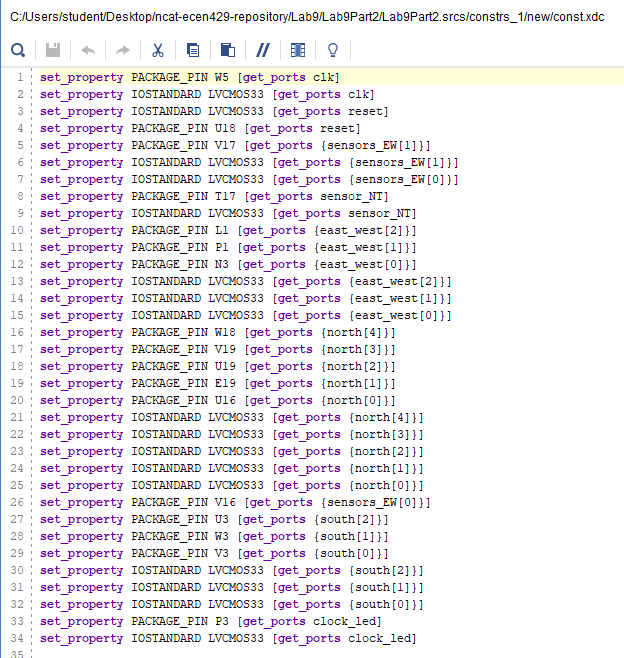
\includegraphics[scale=1]{./images/Part2/l9p2const.png}
	\caption{\label{fig:Prob2Const}Constraints file for Problem 2.}
\end{figure}
\end{center}

\section{Problem 3 VHDL Code}
\begin{lstlisting}[language=VHDL]
library IEEE;
use IEEE.STD_LOGIC_1164.ALL;

entity traffic_control is
    Port ( clk : in STD_LOGIC;
           reset : in STD_LOGIC;
           sensors_EW : in STD_LOGIC_VECTOR(1 downto 0);
           sensor_NT : in STD_LOGIC;
           north : out STD_LOGIC_VECTOR(4 downto 0);
           south : out STD_LOGIC_VECTOR(2 downto 0);
           east_west : out STD_LOGIC_VECTOR(2 downto 0);
           clock_led : out STD_LOGIC;
           output_count : out STD_LOGIC_VECTOR(6 downto 0);
           output_mux : out STD_LOGIC_VECTOR(3 downto 0));
end traffic_control;

architecture Behavioral of traffic_control is

component clock_divider is
     port(clk : in std_logic;
          start_timer : in std_logic;
	  FastClock,MediumClock,SlowClock, led0 : out std_logic);
end component clock_divider;

component traffic_count is
    port(clk, e_signal, w_signal : in STD_LOGIC;
        nt_signal : in STD_LOGIC;
        output_count : out STD_LOGIC_VECTOR(6 downto 0);
        output_mux : out STD_LOGIC_VECTOR(3 downto 0));
end component traffic_count;

signal current_state : STD_LOGIC_VECTOR(3 downto 0) := "0000";
signal next_state : STD_LOGIC_VECTOR(3 downto 0) := "0000";
signal start_timer : STD_LOGIC := '0';
signal fast_clock : STD_LOGIC;
signal medium_clock : STD_LOGIC;
signal slow_clock : STD_LOGIC;
signal sig_count : STD_LOGIC_VECTOR(6 downto 0);
signal sig_mux : STD_LOGIC_VECTOR(3 downto 0);

begin
    clk_div : clock_divider port map(clk, start_timer, fast_clock, 
    medium_clock, slow_clock, clock_led);
    traf_cnt : traffic_count port map(fast_clock, sensors_EW(0), sensors_EW(1), 
    sensor_NT, sig_count, sig_mux);
    
    process(slow_clock, reset)
    begin
        if(reset = '1') then next_state <= "0000";
        elsif(slow_clock'event and slow_clock = '1') then
            case current_state is
                when "0000" =>
                    if(sensors_EW = "01" or sensors_EW = "10"
                     or sensors_EW = "11") then
                        next_state <= "0001";
                    elsif(sensor_NT = '1') then 
                        next_state <= "0111";
                    else
                        next_state <= "0000";
                    end if;
                when "0001" =>
                    next_state <= "0010";
                when "0010" =>
                    next_state <= "0011";
                when "0011" =>
                    if(sensors_EW = "01" or sensors_EW = "10" 
                    or sensors_EW = "11") then
                        next_state <= "0011";
                    else
                        next_state <= "0100";
                    end if;
                when "0100" =>
                    next_state <= "0101";
                when "0101" =>
                    if(sensor_NT = '1') then
                        next_state <= "0110";
                    else
                        next_state <= "0000";
                    end if;
                when "0110" =>
                    if(sensor_NT = '1') then
                        next_state <= "0110";
                    else
                        next_state <= "1001";
                    end if;
                when "0111" =>
                    next_state <= "1000";
                when "1000" =>
                    next_state <= "0110";
                when "1001" =>
                    next_state <= "1010";
                when others =>
                    next_state <= "0000";
            end case;
        end if;
    end process;
    process(current_state)
    begin
        case current_state is
            when "0000" =>
                north <= "00001";
                south <= "001";
                east_west <= "100";
            when "0001" =>
                north <= "01000";
                south <= "010";
                east_west <= "100";
            when "0010" =>
                north <= "10000";
                south <= "100";
                east_west <= "100";
            when "0011" =>
                north <= "10000";
                south <= "100";
                east_west <= "001";
            when "0100" =>
                north <= "10000";
                south <= "100";
                east_west <= "010";
            when "0101" =>
                north <= "10000";
                south <= "100";
                east_west <= "100";
            when "0110" =>
                north <= "00011";
                south <= "100";
                east_west <= "100";
            when "0111" =>
                north <= "00001";
                south <= "010";
                east_west <= "100";
            when "1000" =>
                north <= "00001";
                south <= "100";
                east_west <= "100";
            when "1001" =>
                north <= "00101";
                south <= "100";
                east_west <= "100";
            when others =>
                north <= "00001";
                south <= "100";
                east_west <= "100";
        end case;
    end process;
    current_state <= next_state;
    output_count <= sig_count;
    output_mux <= sig_mux;
end Behavioral;


library IEEE;
use IEEE.STD_LOGIC_1164.ALL;
use IEEE.NUMERIC_STD.ALL;

entity traffic_count is
    port(clk, e_signal, w_signal : in STD_LOGIC;
    nt_signal : in STD_LOGIC;
    output_count : out STD_LOGIC_VECTOR(6 downto 0);
    output_mux : out STD_LOGIC_VECTOR(3 downto 0));
end entity traffic_count;

architecture Behavioral of traffic_count is
signal ew_count : STD_LOGIC_VECTOR(3 downto 0) := "0000";
signal nt_count : STD_LOGIC_VECTOR(3 downto 0) := "0000";

begin
    process(e_signal, w_signal)
    begin
        if(e_signal = '1' or w_signal = '1') then 
        ew_count <= STD_LOGIC_VECTOR(to_unsigned(to_integer(unsigned(ew_count)) + 1, 4));
        end if;
    end process;
    process(nt_signal)
    begin
        if(nt_signal = '1') then nt_count <= 
        STD_LOGIC_VECTOR(to_unsigned(to_integer(unsigned(ew_count)) + 1, 4));
        end if;
    end process;
    
    process(ew_count, nt_count)
    begin
        output_mux <= "0001";
        case ew_count is
            when "0000" =>
                output_count <= "0000001";
            when "0001" =>
                output_count <= "1001111";
            when "0010" =>
                output_count <= "0010010";
            when "0011" =>
                output_count <= "0000110";
            when "0100" =>
                output_count <= "1001100";
            when "0101" =>
                output_count <= "0100100";
            when "0110" =>
                output_count <= "0100000";
            when "0111" =>
                output_count <= "0001111";
            when "1000" =>
                output_count <= "0000000";
            when "1001" =>
                output_count <= "0001100";
            when others =>
                output_count <= "1111111";
        end case;
        output_mux <= "0100";
        case nt_count is
            when "0000" =>
                output_count <= "0000001";
            when "0001" =>
                output_count <= "1001111";
            when "0010" =>
                output_count <= "0010010";
            when "0011" =>
                output_count <= "0000110";
            when "0100" =>
                output_count <= "1001100";
            when "0101" =>
                output_count <= "0100100";
            when "0110" =>
                output_count <= "0100000";
            when "0111" =>
                output_count <= "0001111";
            when "1000" =>
                output_count <= "0000000";
            when "1001" =>
                output_count <= "0001100";
            when others =>
                output_count <= "1111111";
        end case;
    end process;
end Behavioral;
\end{lstlisting}

\section{Problem 3 Constraints File}
\begin{center}
\begin{figure}[H]
	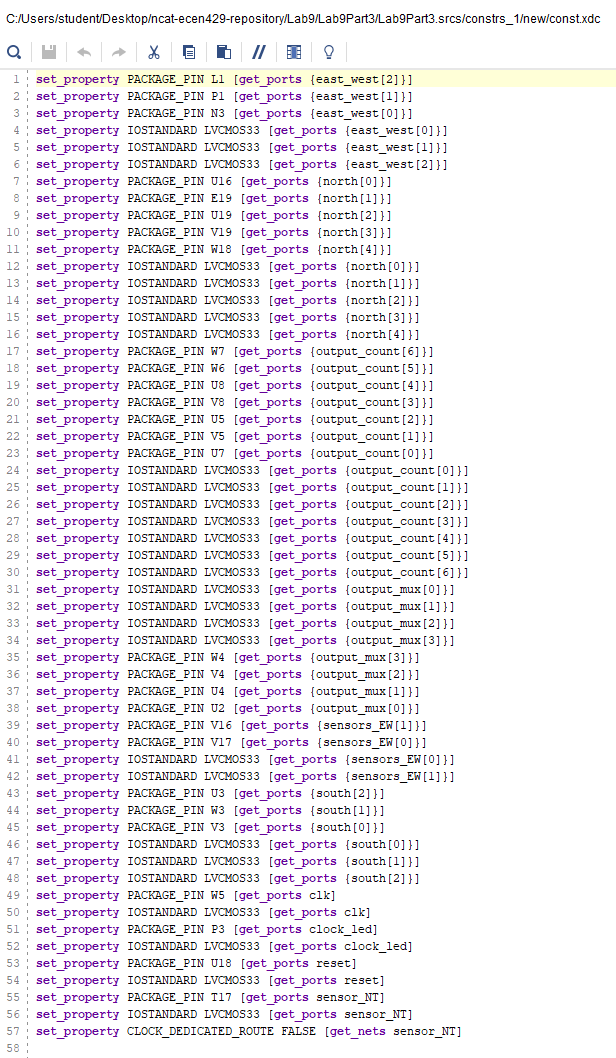
\includegraphics[scale=0.7]{./images/l9p3const.png}
	\caption{\label{fig:Prob3Const}Constraints file for Problem 3.}
\end{figure}
\end{center}

\end{appendices}
\end{document}
